%\documentclass[letterpaper]{IEEEtran}
\documentclass[letterpaper, conference, 11pt]{IEEEtran}      % Use this line for a4 paper

%LatexiDiff ignore tikz:
% $: latexdiff -c "PICTUREENV=(?:picture|tikzpicture|DIFnomarkup)[\w\d*@]*" old.tex new.tex > diff.tex

%\IEEEoverridecommandlockouts                              %

%\usepackage{mathcomSTEP}

%\overrideIEEEmargins 
%\IEEEoverridecommandlockouts                              % This command is only needed if 
% you want to use the \thanks command

%\overrideIEEEmargins                                      % Needed to meet printer requirements.

% See the \addtolength command later in the file to balance the column lengths
% on the last page of the document

%\onecolumn

\usepackage{mathptmx} 
\usepackage{times} 

\usepackage{amsmath} 
\usepackage{amsbsy} 
\usepackage{amssymb}
%\usepackage{newtxtext, newtxmath}
\usepackage{mathrsfs}
\usepackage{comment}
\usepackage[export]{adjustbox}
\usepackage{tikz}
\usetikzlibrary{external,positioning,decorations.pathreplacing,shapes,arrows,patterns}

%\tikzexternalize[mode=list and make]
\usepackage{algorithmicx}
\usepackage{pgfplots}
\usepackage{graphicx}
\usepackage{pstool}
\usepackage[latin1]{inputenc}
\usetikzlibrary{arrows,shapes}
\usepackage{xifthen}
\usepackage{epic}
\usepackage{caption}
\usepackage{epstopdf}

\newtheorem{thm}{\bf{Theorem}}
\newtheorem{cor}[thm]{\bf {Corollary}}
\newtheorem{lem}[thm]{\bf {Lemma}}
\newtheorem{prop}[thm]{\bf {Proposition}}
\newtheorem{example}{\bf {Example}}
\newtheorem{definition}{\bf {Definition}}
\newtheorem{rem}{\bf {Remark}}

\newcommand{\mmse}{\mathsf{mmse}}
\newcommand{\unif}{\mathsf{unif}}
\newcommand{\card}{\mathrm{card}}
\newcommand{\ARE}{\mathsf{ARE}}
\newcommand{\supp}{\mathrm{supp} }
\renewcommand\vec[1]{\ensuremath\boldsymbol{#1}}
\newenvironment{proof}{\paragraph*{Proof}}{\hfill$\square$ \newline}
\newcommand{\sgn}{\mathrm{sgn} }
\newcommand{\argmax}{\mathrm{argmax}}
\newcommand*{\QEDA}{\hfill\ensuremath{\square}}



\tikzstyle{int}=[draw, fill=blue!10, minimum height = 1cm, minimum width=1.5cm,thick ]
\tikzstyle{sint}=[draw, fill=blue!10, minimum height = 0.5cm, minimum width=0.8cm,thick ]
\tikzstyle{sum}=[circle, fill=blue!10, draw=black,line width=1pt,minimum size = 0.5cm, thick ]
\tikzstyle{ssum}=[circle, fill=blue!10,draw=black,line width=1pt,minimum size = 0.1cm]
\tikzstyle{int1}=[draw, fill=blue!10, minimum height = 0.5cm, minimum width=1cm,thick ]
\tikzstyle{enc}=[draw, fill=blue!10, minimum height = 2.7cm, minimum width=1cm,thick ]
\tikzstyle{int}=[draw, fill=blue!10, minimum height = 1cm, minimum width=1.5cm,thick ]


\title{\LARGE \bf Mean Estimation from Single-Bit Measurements}
%
%\author{
%\IEEEauthorblockN{Alon Kipnis}
%\IEEEauthorblockA{Department of Electrical Engineering \\
%Stanford University\\
%Stanford, CA\\}
%\and
%\IEEEauthorblockN{John C. Duchi}
%\IEEEauthorblockA{Department of Statistics \\
%and Department of Electrical Engineering \\
%Stanford University\\
%Stanford, CA\\}
%\and
%\IEEEauthorblockN{Andrea J. Goldsmith}
%\IEEEauthorblockA{Department of Electrical Engineering \\
%Stanford University\\
%Stanford, CA\\}
%}

\begin{document}
\graphicspath{{../Figs/}}
\maketitle
\thispagestyle{empty}
\pagestyle{empty}



%%%%%%%%%%%%%%%%%%%%%%%%%%%%%%%%%%%%%%%%%%%%%%%%%%%%%%%%%%%%%%%%%%%%%%%%%%%%%%%%
\begin{abstract}
We consider the problem of estimating the mean of a symmetric log-concave distribution under the constraint that only a single bit per sample from this distribution is available to the estimator. We study the mean squared error risk in this estimation as a function of the number of samples, and hence number of bits, from this distribution. Under an adaptive scheme in which each bit is a function of the current sample and the previously observed bits, we show that the optimal relative efficiency, compared to the standard mean estimator without bit limitation, is the efficiency of the median. For the distributed scheme we consider the setting where each bit is obtained by comparing against a prescribed threshold value. We show that the maximum likelihood estimator in this case is asymptotically local minimax, and its asymptotic relative efficiency is finite although strictly larger than that of the sample median. 
% and depends on the size of the parameter space from which the mean is taken. Furthermore, assuming a prior on this space, the efficiency in the distributed case approaches $\sigma^2/4f^2(0)$ provided the variance of the distribution is high compared to the variance of the prior. 
%
%Therefore, our results indicates that, rather surprisingly, parametric estimation from the coarsest form of quantization incurs only a multiplicative penalty factor on the number of measurements. For example, this factor is $\pi/2$ for the normal distribution. 
\end{abstract}

%{\color{red}  See LASSO results in http://arxiv.org/abs/1506.02181v1}


%%%%%%%%%%%%%%%%%%%%%%%%%%%%%%%%%%%%%%%%%%%%%%%%%%%%%%%%%%%%%%%%%%%%%%%%%%%%%%%%
\section{Introduction}
\label{sec:Intro}
Estimating parameters from data collected and processed by multiple units may be limited due to communication constraints between these units. 
%
For example, this scenario arises in sensor arrays where information is collected at multiple physical locations and transmitted to a central estimation unit. In these situations, the ability to estimate a particular parameter from the data is dictated not only by the quality of observations and their number, but also by the available bandwidth for communicating between the sensors and the central estimator. The question that we ask is to what extent a parametric estimation task is affected by this constraint on communication, and what are the fundamental performance limits in estimating a parameter subject to such restriction. \\

This paper answers this question in a particular setting: the estimation of the mean $\theta$ of a symmetric log-concave distribution $P_X$ with a finite variance, under the constraint that only a single bit can be communicated on each sample from this distribution. As it turns out, the ability to share information before committing on each single-bit message dramatically affects the performance in estimating $\theta$. We therefore distinguish among three settings:
\begin{itemize}
 \item[(i)] \emph{Centralized} encoding: all $n$ encoders confer and produce a single $n$ bit message. 
 \item[(ii)] \emph{Adaptive} or \emph{sequential} encoding: the $i$th encoder observes the $i$th sample and the $i-1$ previous messages.
 \item[(iii)] \emph{Distributed} encoding: the $i$th message is only a function of the $i$th observation.
 \end{itemize}
Evidently, as far as information sharing is concerned, settings (iii) is a more restrictive version of (ii) which is more restrictive than (i). Below are three application example of each of settings (i)-(iii), respectively:
\begin{itemize}
\item[(i)] {\bf Signal acquisition:} a quantity is measured $n$ times at different instances, and the results are averaged in order to reduce measurement noise. The averaged result is then stored using one of $n$ states. 
\item[(ii)] {\bf analog-to-digital conversion via sigma-delta modulation (SDM):} in SDM an analog signal is converted into a sequence of bits by sampling it at a very high rate and then using one-bit threshold detector combined with a feedback loop to update an accumulated error state. Therefore, the MSE in tracking an analog signal using a SDM falls under our setting (ii) when we assume that the signal at the input to the modulator is a constant (direct current) corrupted by, say, thermal noise \cite{53738}. Since the sampling rates in SDM is usually many times more than the bandwidth of its input, analyzing SDM under a constant input provides meaningful lower bound even for non-constant signals.
\item[(iii)] {\bf Differential privacy:} -- a business entity is interested in estimating the average income of its clients. In order to keep this information as confidential as possible, each client answers a single yes/no questions about its individual income. 
\end{itemize}

We measure the performance in estimating $\theta$ by the mean squared error (MSE) risk. We are interested in particular in the \emph{asymptotic relative efficiency} (ARE) of estimators in the constrained setting compared to asymptotically normal estimators whose variances decreases as $\sigma^2/n+o(n^{-1})$ where $\sigma^2$. Estimator of this form includes the empirical mean of $X_1,\ldots,X_n$, and under some conditions, optimal Bayes estimations. We note that the performance under estimating a signal that may vary with each noisy measurement is always harder that our setting where the parameter (the mean) remains fixed. Therefore, the excess MSE risk due to the one-bit per measurement constraint we derive in this paper can serve as the most optimistic estimate for the degradation in performance in estimating a signal that vary in time. 

% given a prior distribution on the space $\Theta$ where $\theta$ resides. \\

In setting (i), the estimator can evaluate the empirical mean of the samples and then quantize it using $n$ bits. Since the accuracy in describing the empirical mean decreases exponentially in $n$, the error due to quantization is negligible compared to the MSE in estimating the mean. Therefore, the ARE in this setting is $1$. Namely, asymptotically, there is no loss in performance due to the communication constraint under centralized encoding. 
%
In this paper we show that a similar results does not hold even in setting and (ii): the ARE of any adaptive estimation scheme is at least that of the sample median. Specifically, when $P_X$ is normal, this ARE equals $2/\pi \approx 0.637$, showing that the one-bit constraint increases the effective sample size in estimating $\theta$ by at least $2/\pi \approx 1.57$ compared to estimating it without the bit constraint. We also show that this lower bound on the ARE and is tight by providing an estimator that attains it. % This estimator is obtained by averaging the results of a series of comparisons of the samples against certain thresholds. 
%This estimator is can be seen as a stochastic gradient descent procedure for minimizing the absolute error, hence it attains the asymptotic MSE of the sample median. % Interestingly, our estimator attains \eqref{eq:median_MSE} regardless of the particular realization of $\theta$ or the radius of the parameter space from which it is taken.
%
Clearly, the minimal penalty on the MSE in setting (ii) also holds under setting (iii), although the question whether this MSE is achievable (or otherwise, what is the minimal MSE) remains open. Instead, in setting (iii) we restrict ourselves to estimators from messages obtained by comparison against a prescribed value (that may be different for each sample). We show that the maximum likelihood (ML) estimator for $\theta$ from these messages is asymptotically local minimax, and its asymptotic variance is strictly greater than the variance of the median. Thus, at least when limited to threshold detection, the ability to adapt the threshold allows for a more efficient estimation. %This is in contrast to the \\ counterpart of our setting where $\theta$ is taken from a finite space 


Even though the ARE in setting (i) is $1$, this scheme already poses a non-trivial challenge for the design and analysis of an optimal encoding and estimation procedures. Indeed, the standard technique to encode an unknown random quantity using $n$ bits is equivalent to the design of a scalar quantizer \cite{gray1998quantization}. However, the optimal design of this quantizer depends on the distribution of its input, which is the goal of our estimation problem and hence its exact value is unknown. As a result, a non-trivial exploration exploitation trade-off arises in this case. Note that the only missing parameter in our setting is the mean, which, under setting (i), is known to the encoder with uncertainty interval proportional to $\sigma/\sqrt{n}$. Therefore, while it is clear that uncertainty due to quantization decreases exponentially in the number of bits $n$ leading to ARE $1$, an exact expression for the MSE in this setting is still difficult to derive. \par
The situation is even more involved in the adaptive encoding setting (ii): an encoding and estimation strategy that is optimal for $n-1$ adaptive one-bit messages of a sample of size $n-1$, may not lead to a globally optimal strategy upon the recipient of the $n$th sample. Conversely, any one-step optimal strategy, in the sense that it finds the best one-bit message as a function of the current sample and the previous $n-1$ messages, is not guaranteed to be globally optimal. Therefore, while we characterize the optimal detector given the previous messages, this characterization cannot be use to derive a lower bound on the ARE. Instead, our result on the median efficiency being the minimal ARE is obtained by bounding the Fisher information of any $n$ adaptive messages and using the van Trees version of the information inequality \cite{gill1995applications}. 

%Finally, we show that an estimator that attains asymptotic MSE of $\sigma^2\pi/(2n)$ is obtained as a special case of \cite[Thm. 4]{polyak1992acceleration}. In addition to these two results, we also derive the one-step optimal strategy in which the message sent at step $i$th is designed to minimize the MSE given this message and the previous $i-1$ messages. Furthermore, we demonstrates numerically that the MSE under this strategy converges to $\pi \sigma^2/(2n)$.\\ 


\subsection*{Related Works}
As the variance $\sigma^2$ goes to zero, the task of finding $\theta$ using one-bit queries in the adaptive setting (ii) is easily solved by a bisection style method over the parameter space. Therefore, the general case of non-zero variance is a reminiscent of the noisy binary search problem with possibly infinite number of unreliable tests \cite{cicalese2002least, Karp:2007:NBS:1283383.1283478}. However, since we assume a continuous parameter space, a more closely related problem is that of one-bit analog-to-digital conversion of a constant input $\theta$ corrupted by a Gaussian noise. Using a SDM, Wong and Gray \cite{53738} showed that the output of the modulator converges to the true constant input almost surely, so that a SDM provides a consistent estimator for setting (ii). The rate of this convergence, however, was not analyzed and cannot be derived from the results of \cite{53738}. In particular, our results for setting (ii) imply that the asymptotic rate of convergence of the MSE in SDM to a constant input under Gaussian nosie is at most $\sigma^2\pi/2$ over the number of feedback iterations. Baraniuk et. al \cite{baraniuk2017exponential} also considered adaptive one-bit measurements in the context of analog-to-digital conversion, although without noise at the input. Their result of an exponential MSE decaying rate clearly does not hold in the noisy setting (stated otherwise, the MSE can decay exponentially up to the noise level). 
\\

One-bit measurements in the distributed setting (iii) was considered in \cite{904560,4244748, 6882252, chen2010performance, 5184907}, but without optimizing the encoders or their detection rule. % analyzed the estimation from distributed quantized measurements when the same detection rule is applied by all encoders. However, the error criterion considered in these works is the Fisher information rather than the MSE risk or ARE criterion. \par
%Once the decision rule of each encoder is fixed, the optimal estimation of $\theta$ is determined using the maximum a posteriori probability rule. Hence, the distributed setting is reduced to finding the optimal decision rule of each encoder.
The work of \cite{52470} addresses the counterpart of our setting (iii) in the case of hypothesis testing, although the results there cannot be extended to parametric estimation. More generally, when the parameter space $\Theta$ is finite, the characterization of the optimal detection rules was considered by Tsitsiklist in \cite{tsitsiklis1988decentralized}. It was shown there that if the cardinality of $\Theta$ is at most $M$ and the probability of error criterion is used, than no more than $M(M-1)/2$ different detection rules are necessary in order to attain probability of error decreasing exponentially with the optimal exponent. %That is, beyond $M(M-1)/2$ some decision rules can be repeated without lossing optimality.
Furthermore, in a version of this problem for the adaptive sestting \cite{5751320}, it was shown that, with a specific two-stages feedback, there is no gain in feedback compared to the fully distributed setting. Our results implies that the ARE in the distributed setting with threshold detection rules is strictly larger than that in the adaptive setting, suggesting that the case of a finite $\Theta$ is very different than when $\Theta$ is an open set.\par
%
As we explain in details in Section~\ref{sec:preliminary}, the remote multiterminal source coding problem, also known as the CEO problem \cite{berger1996ceo, viswanathan1997quadratic, oohama1998rate, prabhakaran2004rate}, leads to a lower bounds on the MSE in setting (iii). For the case of a Gaussian distribution, this lower bound bounds the ARE to be at most $3/4$. Thus, while this bound on the ARE provides no new information compared to the upper bound of $2/\pi$ we derive for setting (ii), it shows that the distributed nature of the problem is not a limiting factor in achieving MSE close to optimal even under one-bit quantization of each sample.\\

Finally, we note that our settings (ii) and (iii) can be obtained as special cases of 
\cite{zhang2013information} that consider adaptive and distributed estimation protocols for $m$ machines, each has access to $n/m$ independent samples. The main result of \cite{zhang2013information} are bounds on the estimation error as a function of the number of bits $R$ each machine uses for communication. The specialization of their result to our setting, by taking $m=n$ and $R=1$, leads to looser lower bounds then we derive here for cases (ii) and (iii). Other related works include statistical inference under multiterminal data compression \cite{han1987hypothesis, zhang1988estimation}, and one-bit quantization constraints 
%in compressed sensing\cite{baraniuk2017exponential} and 
in MIMO detection in wireless communication \cite{singh2009limits}. \\


\section{Problem Formulation \label{sec:problem}}

\begin{figure}
\begin{center}
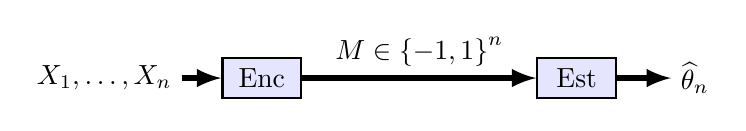
\begin{tikzpicture}[node distance=2cm,auto,>=latex]

\node[node distance = 1.5cm] at (0,0) (source2) {$X_1,\ldots,X_n$};
\node[int1, right of = source2, node distance = 2cm] (enc2) {Enc};  
\draw[->,line width = 2pt] (source2) -- (enc2); 
\node[int1, right of = enc2, node distance = 4cm ] (est) {Est};

\draw[->,line width = 2pt] (enc2) -- node[above, xshift = 0cm] (mes2) {$M \in \left\{-1,1\right\}^n$} (est);   

\node[right of = est, node distance = 1.5cm] (dest) {$\widehat{\theta}_n$};
%         \node [int1] (dec) [right of=dest, node distance = 1.5cm,  align=center] {\small Dec };
%\node [int1] (enc) [right of = dec, node distance = 3cm]{Enc}; 
%\draw[->,line width=2pt] (dec) -- (dest);
\draw[->, line width=2pt] (est) -- (dest);
\end{tikzpicture}
\end{center}
\caption{\label{fig:centralized} Centralized encoding using one bit per sample on average.}
\end{figure}


\begin{figure}
\begin{center}
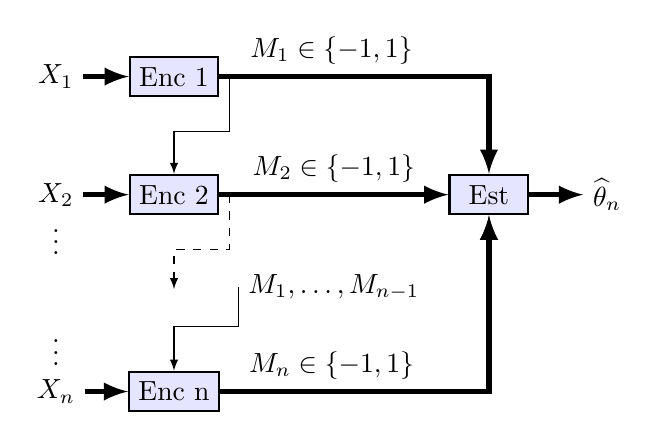
\begin{tikzpicture}[node distance=2cm,auto,>=latex]
  \node at (0,0) (source) {$X_1$} ;
  \node[int1, right of = source, node distance = 1.5cm] (enc1) {Enc 1};  
\draw[->,line width = 2pt] (source) -- (enc1); 

 \node[below of = source, node distance = 1.5cm] (source2) {$X_2$};
\node[int1, right of = source2, node distance = 1.5cm] (enc2) {Enc 2};  
\draw[->,line width = 2pt] (source2) -- (enc2); 

\node[below of = source2, node distance = 2.5cm] (source3) {$X_n$};
\node[int1, right of = source3, node distance = 1.5cm] (enc3) {Enc n};  
\draw[->,line width = 2pt] (source3) -- (enc3); 

\node[below of = source2, node distance = 0.5cm] {$\vdots$};
\node[above of = source3, node distance = 0.6cm] {$\vdots$};
%\node[above of = source3, node distance = 1cm] (dist) {$X_i \sim P_X$};

\node[int1, right of = enc2, node distance = 4cm ] (est) {Est};
\draw[->,line width = 2pt] (enc1) -| node[above, xshift = -2cm] (mes1) {$M_1 \in \left\{-1,1\right\}$} (est);   
\draw[->,line width = 2pt] (enc2) -- node[above, xshift = 0cm] (mes2) {$M_2 \in \left\{-1,1\right\}$} (est);   
\draw[->] (enc1)+(0.7,0) -- +(0.7,-0.7) -| (enc2);

\draw[dashed,->] (enc2)+(0.7,0) -- +(0.7,-0.7) -| +(0,-1.2);
\draw[->,line width = 2pt] (enc3) -| (est);   

\node[below of = mes2, node distance = 1.5cm] (mes3) {$M_1,\ldots,M_{n-1} $};

\draw[->,line width = 2pt] (enc3) -| node[above, xshift = -2cm]  {$M_n \in \left\{-1,1\right\}$} (est);   

\draw[->] (mes3.west) -- +(0,-0.5) -| (enc3);

\node[right of = est, node distance = 1.5cm] (dest) {$\widehat{\theta}_n$};
%         \node [int1] (dec) [right of=dest, node distance = 1.5cm,  align=center] {\small Dec };
%\node [int1] (enc) [right of = dec, node distance = 3cm]{Enc}; 
%\draw[->,line width=2pt] (dec) -- (dest);
\draw[->, line width=2pt] (est) -- (dest);
\end{tikzpicture}
\end{center}
\caption{\label{fig:sequential} Adaptive single-bit encoding: the $i$th encoder delivers a single bit message which is a function of its private sample $X_i$ and the previous messages $M_1,\ldots,M_{i-1}$.}
\end{figure}


\begin{figure}
\begin{center}
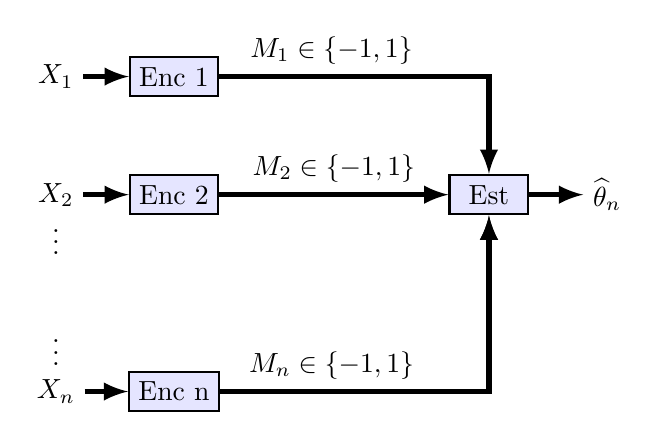
\begin{tikzpicture}[node distance=2cm,auto,>=latex]
  \node at (0,0) (source) {$X_1$} ;
  \node[int1, right of = source, node distance = 1.5cm] (enc1) {Enc 1};  
\draw[->,line width = 2pt] (source) -- (enc1); 

 \node[below of = source, node distance = 1.5cm] (source2) {$X_2$};
\node[int1, right of = source2, node distance = 1.5cm] (enc2) {Enc 2};  
\draw[->,line width = 2pt] (source2) -- (enc2); 

\node[below of = source2, node distance = 2.5cm] (source3) {$X_n$};
\node[int1, right of = source3, node distance = 1.5cm] (enc3) {Enc n};  
\draw[->,line width = 2pt] (source3) -- (enc3); 

%\node[above of = source3, node distance = 1cm] (dist) {$X_i \sim {\mathcal N} \left(\theta, \sigma^2 \right)$};
\node[below of = source2, node distance = 0.5cm] {$\vdots$};
\node[above of = source3, node distance = 0.6cm] {$\vdots$};

\node[int1, right of = enc2, node distance = 4cm ] (est) {Est};
\draw[->,line width = 2pt] (enc1) -| node[above, xshift = -2cm] (mes1) {$M_1 \in \left\{-1,1\right\}$} (est);   

\draw[->,line width = 2pt] (enc2) -- node[above, xshift = 0cm] (mes2) {$M_2 \in \left\{-1,1\right\}$} (est);   

\draw[->,line width = 2pt] (enc3) -| (est);   

\draw[->,line width = 2pt] (enc3) -| node[above, xshift = -2cm]  {$M_n \in \left\{-1,1\right\}$} (est);   

\node[right of = est, node distance = 1.5cm] (dest) {$\widehat{\theta}_n$};
%         \node [int1] (dec) [right of=dest, node distance = 1.5cm,  align=center] {\small Dec };
%\node [int1] (enc) [right of = dec, node distance = 3cm]{Enc}; 
%\draw[->,line width=2pt] (dec) -- (dest);
\draw[->, line width=2pt] (est) -- (dest);
\end{tikzpicture}
\end{center}
\caption{\label{fig:distributed} Distributed single-bit encoding: the single-bit message produced by each encoder is only a function of its private sample $X_i$.}
\end{figure}
Let $\Theta$ be a closed interval of the real line. Let $f(x)$ be a symmetric log-concave density function with a finite second moment $\sigma^2$. We denote by $P_X$ the probability distribution with density $f\left( x-\theta \right)$, where $\theta \in \Theta$. Therefore, $P_X$ is an absolutely continuous log-concave distribution with mean $\theta$, variance $\sigma^2$. Moreover, symmetry and log-concavity of $f(x)$ implies that $P_X$ has a single mode at $x =\theta$. \par
In some cases we assume that $\theta$ is drawn once from the prior distribution $\pi$ on the parameter space $\Theta$. In this cases we assume that $\pi$  
is absolutely continuous distribution, and denote its density by $\pi(\theta)$, i.e., $\pi(d\theta) = \pi(\theta)d\theta$.  
\par
The random variables $X_1,\ldots,X_n$ represent $n$ independent samples from $P_X$. 
We are interested in estimating the parameter $\theta$ from a set of $n$ binary messages $M^n = (M_1,\ldots,M_n)$, obtained from $X^n = (X_1,\ldots,X_n)$ under three possible scenarios: 
\begin{itemize}
\item[(i)~~] Centralized $M^n(X^n)$ (Fig.~\ref{fig:centralized}).
\item[(ii)~] Adaptive $M_i(X_i,M^{i-1})$, $i=1,\ldots,n$ (Fig.~\ref{fig:sequential}).
\item[(iii)] Distributed $M_i(X_i)$, $i=1,\ldots,n$ (Fig.~\ref{fig:distributed}).
\end{itemize}

The performance of an estimator $\hat{\theta}_n \triangleq \hat{\theta}_n(M^n)$ in any of these cases is measured according to the mean squared error (MSE) risk:
\begin{equation}
\label{eq:error_def}
R_n \triangleq \mathbb E\left(\hat{\theta}_n - \theta \right)^2,
\end{equation}
where the expectation is taken with respect to the distribution of $X^n$ and the prior distribution $\pi(\theta)$.  
%It is well known that minmax estimation error 
%\begin{equation}
%R_n = \min \sup_{\theta \in \Theta}  \mathbb E\left[ \left(\hat{\theta}_n - \theta \right)^2 | \theta \right],
%\end{equation}
%can be obtained from $R_n$ by assuming a particular least favorable prior distribution on the parameter space $\Theta$ \cite{casella1981}. 
%
The main problem we consider is the minimal value of \eqref{eq:error_def} as a function of $n$, under various choices of the encoding functions in cases (i), (ii), and (iii). \\

Particular interest is given to the ARE of estimators with respect to an asymptotically normal efficient estimator without the one-bit constraint. Specifically,  let $\{a_n,\,n\in \mathbb N\}$ be a sequence such that 
\[
\sqrt{a_n}\left(\hat{\theta}_n - \theta\right) \overset{D}{\longrightarrow} \mathcal N(0, \sigma^2).
\]
Then the ARE of $\hat{\theta}_n$ with respect to an unconstrained efficient estimator for $\theta$ is defined as \cite[Def. 6.6.6]{lehmann2006theory}
\[
\ARE(\hat{\theta}_n) \triangleq
\lim_{n\rightarrow \infty} \frac{a_n}{n}. 
\]
Note that in the special case where there exists $V \in \mathbb R$ such that
\[
a_n \mathbb E \left(\hat{\theta}_n - \theta \right)^2 = V + O(1/n),
\]
then the ARE of $\hat{\theta}_n$ is finite and equals $\sigma^2/V$. 
%sample mean $\bar{X}_n = \frac{1}{n} \sum_{i=1}^n X_i$. Since the MSE attained by the latter is $\sigma^2/n$, this relative efficiency is defined as
%\begin{equation}
% \lim_{n \rightarrow \infty} \frac{n}{\sigma^2}  R_n. 
%\label{eq:relative_efficiency}
%\end{equation}

%In addition to the notations defined above, we denote by $\phi(x)$ the standard normal density and by $\Phi(x)$ the standard normal cumulative distribution function. Prime denote derivative with respect to $\theta$.

\section{Preliminary Results \label{sec:preliminary}}
On a first impression it may not be clear whether consistent estimation of the mean is even possible in the adaptive and centralized settings. On the other hand, one may suspect that estimation in these cases is trivial as in the centralized setting (i), where it is easy to attain ARE 1. In this section we settle this skepticism by showing that (1) a consistent estimator with an asymptotically normal distribution always exists in setting (iii), and (2) the ARE in setting (iii) with $P_X = \mathcal N(\theta, \sigma^2)$ is bounded from below by $3/4$. 

\subsection{Consistent Estimation}
Denote by $M_i$ is the indicator of the event $X_i > \theta_0$ for some arbitrary $\theta_0$. Note that
\[
\frac{1}{n} \sum_{i=1}^n M_i \overset{a.s.}{\rightarrow} F(\theta),
\]
where $F(x)$ is the cumulative distribution of $X_1-\theta$ that is assumed to be known. Therefore, 
\begin{equation}
\label{eq:estimator_naive}
\hat{\theta}_n = F^{-1}\left( \frac{1}{n} \sum_{i=1}^n M_i \right)
\end{equation}
is a consistent estimator for $\theta$ under setting (iii). Moreover, it can be verified, as we do in Section~\ref{sec:distributed}, that $\hat{\theta}_n$ is asymptotically normal with variance that is the inverse of
\begin{equation} \label{eq:eta_def}
\eta(\theta-\theta_0) \triangleq \frac{f^2(\theta-\theta_0)} {F(\theta-\theta_0)\left(1-F(\theta-\theta_0)\right)}. 
\end{equation}
In particular, the ARE of $\hat{\theta}_n$ is finite and equals $\sigma^2/\eta(\theta - \theta_0)$. For $f(x)$ the normal density, it is shown in \cite{Samford1953} and \cite{hammersley1950estimating} that the function $\eta(x)$ is a strictly decreasing function of $|x|$. The following proposition, generalizes this property of $\eta(x)$ to any log-concave distribution.
\begin{prop} \label{prop:eta}
Let $f(x)$ be log-concave, symmetric and differntiable probability density function. Then 
\begin{itemize}
\item[(i)] The function
\[
\eta(x) = \frac{f^2(x)}{F(x) \left(1-F(x) \right)}
\]
is symmetric and strictly decreasing for any $x>0$ in the support of $f(x)$. In particular, $
\eta(x) \leq \eta(0) = 4f^2(0)$. 
\item[(ii)] $\eta(x)$ goes to $0$ as $|x|$ goes to infinity. 
\end{itemize}

\end{prop}
\begin{proof}
See Appendix~\ref{app:proofs}. 
\end{proof}
%
\begin{figure}
\begin{center}
\begin{tikzpicture}[scale = 0.6]
\begin{axis}[
width=8cm, height=6cm,
xmin = -3, xmax=3, 
restrict y to domain = 0:100,
ymin = 0,
samples=10, 
xlabel= $x$,
xtick={-2,-1,0,1,2},
xticklabels={-2,-1,0,1,2},
ytick={0,0.3989423,0.6366198},
yticklabels={0,$\frac{1}{\sqrt{2 \pi}}$,$2/\pi$},
line width=1.0pt,
mark size=1.5pt,
ymajorgrids,
xmajorgrids,
legend style= {at={(1,1)},anchor=north east,draw=black,fill=white,align=left}
]
\addplot[color = blue, solid, smooth] plot table [x = x, y = y, col sep=comma] {../Figs/eta.csv};
\addlegendentry{$\eta(x)$};
\addplot[domain = -5:5, samples = 50, color = red, solid, smooth]  {exp(-x^2/2) / sqrt(2*3.14159)};
\addlegendentry{$\phi(x)$};
\end{axis}
\end{tikzpicture}
%
\begin{tikzpicture}[scale = 0.6]
\begin{axis}[
width=8cm, height=6cm,
xmin = -4, xmax=4, 
restrict y to domain = -10:0,
ymin = -10,
samples=10, 
xlabel= $x$,
xtick={-3,-2,-1,0,1,2,3},
xticklabels={-3,-2,-1,0,1,2,3},
ytick={0,-0.45158,-0.919},
yticklabels={0,,},
line width=1.0pt,
mark size=1.5pt,
ymajorgrids,
xmajorgrids,
legend style= {at={(1,1)},anchor=north east,draw=black,fill=white,align=left}
]
\addplot[color = blue, solid, smooth] plot table [x = x, y = logy, col sep=comma] {../Figs/eta.csv};
\addlegendentry{$\log \eta(x)$};
\addplot[domain = -5:5, samples = 30, color = red, solid, smooth]  {-(x)^2/2 -0.9189};
\addlegendentry{$\log \phi(x)$};
\end{axis}
\end{tikzpicture}
\caption{
The function $\eta(x) = f^2(x) / F(x)F(-x)$ (blue) for $f(x) = \phi(x)$ the standard normal density (red).
\label{fig:eta}
}
\end{center}
\end{figure}

At $\theta = \theta_0$ the variance of $\hat{\theta}_n$ of \eqref{eq:estimator_naive} equals $1/(4f(0)^2)$ which is the variance of the median. However, since  $\eta(x)$ vanishes as $|x|\rightarrow \infty$ (see illustration in Fig.~\ref{fig:eta} for the normal density),  the variance of $\hat{\theta}_n$ may be very large when $\theta$ is away from $\theta_0$. In this case, the estimator $\hat{\theta}_n$ has little practical value unless $\Theta$ is very small compared to $\sigma^2$. \par
%
In Section~\ref{sec:sequential} we present an asymptotically normal estimator that attains the variance of the median $1/\eta(0)$ regardless of the radius of $\Theta$ or the prior $\pi(\theta)$. We also show in Section~\ref{sec:sequential} that no estimator can attain variance that is smaller than $1/\eta(0)$, so that the ARE of any estimator is at least $\sigma^2\eta(0) = (2f(0)\sigma)^2$. 

\subsection{Lower bound from the CEO \label{sec:ceo}}
The CEO setting includes $n$ encoders, each has access to a noisy version of a random source sequence \cite{berger1996ceo}. 
% $\left\{ U_j,\,j=1,2,\ldots \right\}$. 
The $i$th encoder observes $k$ noisy source symbols and transmit $R_i k$ bits to a central estimator. \par
Assuming that $\theta$ is drawn once from the prior $\pi(d\theta)$, our mean estimation problem from one-bit samples under distributed encoding (setting (iii) in the Introduction) corresponds to the Gaussian CEO setting with $k=1$ source realization: the $i$th encoder uses $R_i=1$ bits to transmit a message that is a function of $X_i = \theta + \sigma Z_i$, where $Z_i$ is standard normal. As a result, a lower bound on the MSE distortion in estimating $\theta$ in the distributed encoding setting is given by the MSE in the optimal source coding scheme for the CEO with: $n$ terminals of codes rates $R_1 = \ldots = R_n = 1$, a Gaussian observation noise at each terminal of variance $\sigma^2$, and an arbitrary number of $k$ independent draws of $\theta$. Note that the difference between the CEO and ours lays in the privilege of each of the CEO encoders to describe $k$ realizations of $\theta$ using $k$ bits with MSE averaged over these realization, whereas our setting only allows $k=1$. 
 \\

By using an expression for the minimal MSE in the Gaussian CEO as the number of terminals goes to infinity, we conclude the following:
\begin{prop} \label{prop:ceo_lower_bound}
Assume that $\Theta = \mathbb R$ and that $\pi(\theta) = \mathcal N(0,\sigma_\theta^2)$. Then any estimator $\hat{\theta}_n$ of $\theta$ in the distributed setting satisfies
\begin{equation} \label{eq:ceo_bound}
 n\mathbb E \left( \theta - \theta_n \right)^2 \geq \frac{4\sigma^2}{3} + O(n^{-1}),
\end{equation}
where the expectation is with respect to $\theta$ and $X^n$.
\end{prop}

\begin{proof}
We consider the expression \cite[Eq. 10]{chen2004upper} that gives the minimal distortion $D^\star$ in the CEO with $L$ observers and under a total sum-rate $R_\Sigma = R_1 + \ldots +R_L$:
\begin{equation} \label{eq:ceo_optimal_sumrate}
R_{\Sigma} = \frac{1}{2} \log^+ \left[ \frac{\sigma_\theta^2}{D^\star} \left( \frac{D^\star L}{ D^\star L - \sigma^2 + D^\star \sigma^2 / \sigma_\theta^2 }\right)^L  \right].
\end{equation}
Assuming $R_\Sigma = n$ and $L=n$, we get
\begin{equation} \label{eq:ceo_optimal_sumrate}
n = \frac{1}{2} \log_2 \left[ \frac{\sigma_\theta^2}{D^\star} \left(\frac{ D^\star n }{D^\star n - \sigma^2 + D^\star \sigma^2/\sigma_\theta^2 }  \right)^n  \right].
\end{equation}
The value of $D^\star$ that satisfies the equation above describes the MSE under an optimal allocation of the sum-rate $R_\Sigma = n$ among the $n$ encoders. Therefore, $D^\star$ provides a lower bound to the CEO distortion with $R_1=\ldots,R_n = 1$ and hence a lower bound to the minimal MSE in estimating $\theta$ in the distributed encoding setting. By considering $D^\star$ in \eqref{eq:ceo_optimal_sumrate} as $n\rightarrow \infty$, we see that 
\[
D^\star = \frac{ 4\sigma^2 }{3n + 4 \sigma^2 / \sigma_\theta^2 } + o(n^{-1}) =  \frac{4\sigma^2}{3n} + o(n^{-1}). 
\]
\end{proof}
We note that although the lower bound \eqref{eq:ceo_bound} was derived assuming the optimal allocation of $n$ bits per observation among the encoders, this bound cannot be tightened by considering the CEO distortion while enforcing the condition $R_1=\ldots = R_n = 1$. Indeed, an upper bound for the CEO distortion under the condition $R_1=\ldots = R_n = 1$ follows from \cite{KipnisRini2017}, and leads to
\[
D^\star \leq  \left( \frac{1}{\sigma_\theta^2} +  \frac{3n}{4\sigma^2 + \sigma_\theta^2} \right)^{-1}   =
\frac{4 \sigma^2}{3n} +  \frac{\sigma_\theta^2}{3n} + O(n^{-2}),
\]
which is equivalent to \eqref{eq:ceo_bound} when $\sigma_\theta$ goes to zero. \par
From the formulation of the CEO problem, it follows that the difference between the MSE lower bound \eqref{eq:ceo_bound} and the actual MSE in the distributed setting (case (iii)) is exclusively attributed  to the ability to perform coding over blocks. Namely, each CEO encoder may encode an arbitrary number of $k$ independent realizations of $\theta$ using $k$ bits, versus only one realization with one bit in ours. In other words, it is the ability to exploit the geometry of a high-dimensional product probability space that 
distinguishes between the CEO problem with one bit per encoder and the mean estimation problem from one-bit measurements in the distributed setting of Fig.~\ref{fig:distributed}. 

\section{Adaptive Estimation \label{sec:sequential}}
The first main results of this paper, as described in Theorem~\ref{thm:adpative_lower_bound} below, states that the ARE of any adaptive estimator cannot be larger than $(2f(0)\sigma)^2$, which the ARE of the median of $X^n$. Next, we provide a particular adaptive estimation scheme that attains this maximal efficiency. Finally, in Theorem~\ref{thm:opt_one_step}, we provide an adaptive estimation scheme that is one-step optimal in the sense that at each step $i$, the message $M_i$ that minimizes the MSE given $X_i$ and the previous $M^{i-1}$ messages is chosen. Numerical simulations for the case of $f(x)$ the normal density function shows that the ARE of the estimator described by this scheme is $(2f(0)\sigma)^2$. 

\subsection{Maximal efficiency of adaptive one-bit schemes}
Our first results asserts that the ARE of any adaptive estimation scheme is bounded from above by $(2 f(0)\sigma )^2$, as follows from the following theorem:
\begin{thm}[minimal relative effeciency] \label{thm:adpative_lower_bound}
Let $\hat{\theta}_n$ be any estimator of $\theta$ in the adaptive setting of Fig.~\ref{fig:sequential} and assumes that $\pi(\theta)$ converges to zero at the endpoints of the interval $\Theta$. Then
\[
\mathbb E\left[ (\theta-\theta_n)^2 \right] \geq  \frac{\pi \sigma^2 }{2n +\pi \sigma^2  I_0}  =  \frac{\sigma^2}{4f^2(0) n}+o(n^{-1}),
\]
where 
\[
I_0 = \mathbb E \left( \frac{d}{d\theta} \log \pi (\theta) \right)^2
\]
is the Fisher information with respect to a location model in $\theta$. 
\end{thm}

\subsubsection*{Sketch of Proof}
The main idea in the proof is to bound from above the Fisher information of any set of $n$ single-bit messages with respect to $\theta$. Once this bound is achieved, the result follows by using the van-Trees inequality \cite[Thm. 2.13]{tsybakov2008introduction},\cite{gill1995applications} which bounds from below the MSE of any estimator of $\theta$ by the inverse of the expected value of the aforementioned Fisher information plus $I_0$. The details are given in the Appendix.\\

Next, we present an adaptive estimation scheme that attains the maximal ARE of $(2f(0)\sigma)^2$. 

\subsection{Asymptotically optimal estimator}
Let $\left\{ \gamma_n,\, n\in \mathbb N \right\}$ be a strictly positive sequence. Consider the following estimator $\hat{\theta}_n$ for $\theta$:  
\begin{equation}
\label{eq:sgd_alg}
\theta_n = \theta_{n-1} +  \gamma_n \sgn (X_n - \theta_{n-1}), \quad n = 1,2,\ldots,
\end{equation}
and set the $n$th step estimation as
\begin{equation} \label{eq:sgd_est}
\hat{\theta}_n =  \frac{1}{n} \sum_{i=1}^n  \theta_i. 
\end{equation}

For the estimator defined by \eqref{eq:sgd_alg} and \eqref{eq:sgd_est} we have the following results:
\begin{thm} \label{thm:sgd}
Consider the sequence $\left\{\hat{\theta}_n,\, n\in \mathbb N \right\}$ defined by \eqref{eq:sgd_est}. 
\begin{enumerate}
\item[(i)] Assume that $\left\{ \gamma_n,\, n\in \mathbb N \right\}$ satisfies
\begin{equation} \label{eq:conditions1}
\begin{cases}
\frac{\gamma_n - \gamma_{n+1}}{\gamma_n} = o(\gamma_n), &  \\
\sum_{n=1}^\infty \frac{\gamma_n^{(1+\lambda)/2}} {\sqrt{n}} < \infty, & 
\mathrm{for~some~}0< \lambda \leq 1
\end{cases}
\end{equation}
(e.g., $\gamma_n = n^{-\beta}$ for $\beta \in (0,1)$). Then
\[
\sqrt{n} \left( \hat{\theta}_n - \theta \right) \overset{d}{\rightarrow} \mathcal N \left(0,  \left( 2 f(0)\right)^{-2} \right).
\]
\item[(ii)] Assume that in addition to \eqref{eq:conditions1}, $\left\{ \gamma_n,\, n\in \mathbb N \right\}$ satisfies
\begin{equation} \label{eq:conditions2}
\begin{cases}
\gamma_n = o(n^{-2/3}), &  \\
\sum_{n=1}^\infty \gamma_n = \infty.  & \\
\end{cases}
\end{equation}
(e.g., $\gamma_n = n^{-\beta}$ with $2/3<\beta<1$). Then
\[
\lim_{n\rightarrow \infty} n\mathbb E \left[ \left(\theta-\hat{\theta}_n \right)^2 \right] = \left( 2 f(0)\right)^{-2}. 
\]
\end{enumerate}
\end{thm}

\subsubsection*{Proof}
The asymptotic behavior of \eqref{eq:sgd_est} is obtained from \cite[Thm. 4]{polyak1992acceleration} and \cite[Thm. 2]{polyak1990new}. The details are in the Appendix.\\

Theorem~\ref{thm:sgd} implies that the estimator $\hat{\theta}_n$, defined by \eqref{eq:sgd_est} and \eqref{eq:sgd_alg}, attains the maximal ARE as established by Theorem~\ref{thm:adpative_lower_bound}.
\par
Note that $\theta_0$ is not explicitly defined 
in equation \eqref{eq:sgd_est}. A reasonable initialization for $\theta_0$ is $\theta_0 = \mathbb E [\theta]$, although Theorem~\ref{thm:sgd} implies that the asymptotic behavior of the estimator is indifferent to this initialization. Thus, the optimal efficiency is attained regardless of the prior distribution on $\theta$ or the radius of the parameter space $\Theta$. Nevertheless, the bound in Theorem~\ref{thm:adpative_lower_bound} suggests that the non-asymptotic MSE can be reduced significantly whenever the location information $I_0$ is large. In what follows, we consider a greedy estimation procedure that uses the optimal decision rule given the prior distribution and the previous messages. In particular, this procedure exploit the prior information on $\theta$ provided by its prior. 

\subsection{One-step optimal estimation}
We now consider an estimation scheme that posses the property of \emph{one-step optimality}: at each step $n$, the $n$th encoder designs the detection region $M_n^{-1}(1)$ such that the MSE given $M^n$ is minimal. In other word, this scheme designs the messages in a greedy manner, such that the MSE at step $n$ is minimal given the current state of the estimation described by $M^{n-1}$. \\

The following theorem determine the message, i.e., the decision rule $(M^{n-1},X_n)\rightarrow M_n$, that minimizes the next step MSE:
\begin{thm}[optimal one-step estimation] \label{thm:opt_one_step}
Let $\pi(\theta)$ be an absolutely continuous log-concave probability distribution. Given a sample $X$ from a log-concave distribution with mean $\theta$, define 
\begin{equation}
\label{eq:adaptive_main_message}
M^\star = \sgn(X - \tau),
\end{equation}
where $\tau$ satisfies the equation
\begin{equation}
 \label{eq:fixed_point}
 \tau = \frac{m^-(\tau) + m^+(\tau)}{2},
\end{equation}
with
\begin{align*}
m^-(\tau)  & = \frac{\int_{-\infty}^{\tau} \theta \pi(d\theta) }{\int_{-\infty}^{\tau} \pi(d\theta)} ,\\
m^+(\tau) & = \frac{\int_{\tau}^\infty \theta \pi(d\theta) }{\int_{\tau}^\infty \pi(d\theta)} .
\end{align*}
Then for any estimator $\hat{\theta}$ which is a function of $M(X) \in \{-1,1\}$, we have
\begin{equation}
\label{eq:opt_cond}
\mathbb E \left(\theta-\hat{\theta}(M)\right)^2 \geq  \mathbb E \left(\theta- \mathbb E[\theta|M^\star]\right)^2,
\end{equation}
\end{thm}

\begin{proof}
The proof is completed by the following two lemmas, proofs of which can be found in the Appendix:
\begin{lem} \label{lem:unique}
Let $f(x)$ be a log-concave probability density function. Then the equation 
\begin{equation}
\label{eq:lem_fixed_point}
2x = \frac{\int_x^\infty uf(u)du}{\int_x^\infty f(u)du} + \frac{\int_{-\infty}^x uf(u)du}{\int_{-\infty}^x f(u)du} 
\end{equation}
has a unique solution.
\end{lem}
\begin{lem} \label{lem:adaptive}
Let $U$ be an absolutely continuous random variable with pdf $P(du)$. Then the one-bit message $M^\star\in \{-1,1\}$ that minimizes
\[
\int \left( u - \mathbb E[U|M(u)]  \right)^2 P(du)
\]
is given by
\[
M^\star  =  \sgn(U - \tau),
\]
where $\tau$ is the unique solution to
 \[
2 \tau = \frac{\int_{\tau}^\infty u P(du)} {\int_{\tau}^\infty P(du)} + \frac{\int_{-\infty}^{\tau} u P(du)}{\int_{-\infty}^{\tau} P(du)}.
\]
\end{lem}
\end{proof}

\begin{rem}
The value of the optimal threshold as given in Theorem~\ref{thm:opt_one_step} is different than the one given in \cite[Eq. 5]{1619423} for apparently the same problem. Indeed, it seems like Equation 4 there is erroneous. 
\end{rem}

By applying at each step the optimal one-step decision rule from Theorem~\ref{thm:opt_one_step},  we arrive at the following adaptive encoding and estimation scheme: 
\begin{itemize}
\item Initialization: set $P_0(t) = \pi(t)$ and $\tau_0 = \mathbb E \theta$. 
\item For $n\geq 1$:
\begin{enumerate}
\item[(1)] Update the prior as
\begin{align}
& P_n(t) = P(\theta=t |M^n) \nonumber \\
& \quad = \frac{ P\left( \theta=t | M^{n-1} \right) P(M_n | \theta = t , M^{n-1})  } { P(M_n | M^{n-1} )} \nonumber \\ 
& \quad = \alpha_n  P_{n-1}(t) F\left(M_n (t - \tau_{n-1}) \right), \label{eq:density_update}
\end{align}
where $\alpha_n$ is given by
\[
\alpha_n = \left(\int_{\mathbb R} P_{n-1}(t) F \left(M_n (t- \tau_{n-1}) \right)  dt \right)^{-1}. 
\]
\item[(2)] The $n$th estimate for $\theta$ is the conditional expectation of $\theta$ given $M^n$, namely
\begin{equation}
\theta_n = \mathbb E \left[ \theta| M^n\right] = \int_{-\infty}^\infty t P_n(t) dt. \label{eq:estimator_update}
\end{equation}
\item[(3)] Obtain $\tau_n$ from equation \eqref{eq:fixed_point} with the updated prior $P_n(t)$. Note that $F(x)$ is log-concave so the updated prior $P_n(t)$ remains log-concave and thus a unique solution to \eqref{eq:fixed_point} is guaranteed by Lemma~\ref{lem:unique}. 
\item[(4)] Update the $(n+1)$th message as
\begin{equation}\label{eq:message_update}
M_{n+1} = \sgn(X_{n+1}-\tau_n)
\end{equation}
\end{enumerate}
\end{itemize}
Since equation \eqref{eq:fixed_point} has no analytic solution in general, it is hard to derive the asymptotic behavior of the estimator defined by \eqref{eq:estimator_update} and \eqref{eq:message_update}. We conjecture, however, that it attains the asymptotic relative efficiency of $4f^2(0)$ under the same conditions on $f(x)$ in the problem formulation. 
In Fig.~\ref{fig:adaptive_error} we demonstrate this convergence in the case where $f(x)$ is the standard normal density. Also shown in Fig.~\ref{fig:adaptive_error} are the normalized MSE of the asymptotically optimal estimator defined by \eqref{eq:sgd_alg} and \eqref{eq:sgd_est}, as well as the MSE achieved by the sample mean for the same sample realization. 

\begin{figure}
\begin{center}
\begin{tikzpicture}
\node at (0,0) {\includegraphics[scale=0.4]{one_bit_adpative}};
%\node[color = blue,  minimum width=1cm, align = left] at (1.5,1.5) {assymptotically optimal \eqref{eq:sgd_est}};
%\node[color = red, minimum width=1cm, align = left] at (1.5,0.55) {one-step optimal \eqref{eq:message_update}} ;
\node[rotate = 90, scale = 0.7] at (-3.8,0) {$n \mathbb E \left(\hat{\theta}_n - \theta \right)^2$};
\node[scale = 0.7] at (0,-2.4) {$n$};
%\draw[dashed] (-3.5,1.18) node[left, scale = 0.7] {$\frac{\pi}{2}$}-- (-3,1.18);
\end{tikzpicture}
\caption{Normalized empirical risk $n\left(\hat{\theta}_n-\theta\right)^2$ versus number of samples $n$ for $500$ Monte Carlo trials. In each trial, $\theta$ is chosen uniformly in the interval $(-3,3)$. \label{fig:adaptive_error}  }
\end{center}
\end{figure}


\begin{comment}
\subsection{Relation to Sigma-Delta Modulation \label{subsec:sdm}}
The SDM is a device that converts continuous-time analog signals to a discrete-time sequence of binary digits. The basic operation of a SDM can be described as follows: the modulator takes as input a sequence of continuous amplitude samples $X_n$, which are typically represents samples of a continuous-time signal taken uniformly at sampling rate $f_s$ much higher than the Nyquist rate of the signal \cite{1095151}. The output of the modulator is a sequence $M_n$ of binary values, obtained according to the following rule: 
\begin{align}
\begin{cases} V_{n+1} & =  V_n - \alpha q(V_n) + X_n, \\
M_n & = \sgn(V_n)  \end{cases}, \quad n=1,2,\ldots, \label{eq:sdm}
\end{align}
where $\alpha > 0$ is a parameter of the modulator that is determined by the maximal value of the input sequence $X^n$. The SDM of the form \eqref{eq:sdm} was studied in \cite{53738} under the assumption that the input process $X_n$ is an i.i.d Gaussian process. The main results from \cite{53738} shows that regardless of the initial state $V_0$, the process $M_n$ is a stationary ergodic process with mean $\theta$. It follows that a consistent estimation of $\theta$ is obtained by taking the mean of the sequence $\{M_n\}$. However, the results from \cite{53738} does not provide a closed form for the second order statistics of $\{M_n\}$, so that convergence rate cannot be derived from \cite{53738}.  
\end{comment}


\section{Distributed Estimation from Threshold Detectors \label{sec:distributed}}
We now consider the distributed encoding setting described in Fig.~\ref{fig:distributed}, in which each single-bit message is independent of the other messages. Instead of searching for the optimal choice of the messages, we only consider messages that are obtained each sample against a prescribed threshold. Namely, each message is of the form
\begin{equation}
\label{eq:threshold_message}
M_i = \sgn(t_i - X_i) = \begin{cases} 1 & X_i< t_i, \\
-1 & X_i > t_i,
\end{cases}  
\end{equation}
where $t_i\in\mathbb R$ is the \emph{threshold} of the $i$th detector applied by the encoder on it sample $X_i$. The \emph{density} $\lambda_n$ of the set of threshold values $\mathcal T_n  \triangleq \left\{t_1,\ldots,t_n \right\}$ is defined as their empirical distribution, i.e., for an interval $I \subset \mathbb R$, 
\[
\lambda_n(I) = \frac{ \card \left( \mathcal T_n \cap I \right)}{n}.
\]
We further assume that $\lambda_n$ converges (weakly) to a probability measure $\lambda(dt)$ on $\mathbb R$. For example, this convergence occurs whenever $t_1,\ldots,t_n$ are drawn independently from the probability distribution $\lambda(dt)$. 
 \\

\subsection{Local Asymptotic Minimax Estimation}

In order to estimate $\theta$ from the messages $M^n$, we consider the maximum likelihood (ML) estimator. The log-likelihood function of $\theta$ is given by
\[
l(M^n  |\theta ) =  \sum_{i=1}^n \log F \left( M_i \left( t_i - \theta \right) \right). 
\]
Since $F(x)$ is a log concave function, the log-likelihood function has a unique maximizer $\hat{\theta}_n$ which is the ML estimator. Specifically, the ML estimator $\hat{\theta}_{ML}$ is the unique root of 
\[
\sum_{i=1}^n M_i \frac{f \left( t_i-\theta\right) }{F \left(M_i  (t_i-\theta)\right) } 
\]

Next, we show that under the assumptions above the sequence of messages $M^n$ defines a local asymptotic normal (LAN) family of probability distributions. As a result, we conclude that the ML estimator in estimating $\theta$ from $M^n$ satisfies a local asymptotic minimax property with respect to the \emph{precision} parameter of this LAN family \cite{van2000asymptotic}. 
\begin{thm} \label{thm:LAN}
Let $f(x)$ be a log-concave, symmetric, and twice differentiable probability density function. Consider the sequence $M^n$ of threshold detectors 
\[
M_i = \sgn(X_i - t_i),\quad i=1,\ldots,n,
\]
with threshold density converges to a probability measure $\lambda$. The the following two statements hold:
\begin{itemize}
\item[(i)] Any estimator ${\theta}_n$ of $\theta$ which is a function of $M^n$ satisfies
\[
\liminf_{c\rightarrow \infty}\, \liminf_{n\rightarrow \infty} \sup_{\tau\,:\,| \tau - \theta| \leq \frac{c}{\sqrt{n}} }  n \mathbb E \left({\theta}_n - \tau \right)^2 \geq 1/K(\theta),
\]
where 
\[
K(\theta) \triangleq \int \eta\left(t-\theta \right) \lambda(dt),
\]
and 
\[
 \eta(x) \triangleq \frac{ f^2\left( x \right)}{ F\left( x \right) \left(1-F(x) \right)}. 
\]
\item[(ii)] The asymptotic distribution of the ML estimator $\hat{\theta}_n$ is given by
\[
\sqrt{n}(\hat{\theta}_n - \theta) \overset{D}{\rightarrow} \mathcal N\left(0,1/K(\theta) \right).
\]
\end{itemize}
\end{thm}

\begin{rem}
The condition that $\lambda_n(dt)$ converges weakly to $\lambda(dt)$ can be relaxed to the condition that for any $\theta \in \Theta$, 
\[
\frac{1}{n} \sum_{i=1}^n  \eta \left( t_i-\theta \right)  
\]
converges to $K(\theta)$.
\end{rem}

\begin{proof}
See Appendix. 
\end{proof}

It follows from Theorem~\ref{thm:LAN} that the asymptotic MSE of the ML estimator is $1/(nK(\theta))$, and that this MSE is asymptotically minimal with respect to all local alternative estimators for $\theta$. In particular, we conclude that the ARE of any estimator based on threshold detection is $K(\theta)\sigma^2$. \par
It follows from Proposition~\ref{prop:eta} that $\eta(x)$ attains its maximum at the origin. Since the thresholds density $\lambda$ integrates to $1$, it follows that
\[
K(\theta) \leq \sup_{t\in \mathbb R} \eta \left( t-\theta\right)  = \eta(0) = 4f^2(0).
\]
This upper bound on $K(\theta)$ implies that the ARE of any distributed estimator is not smaller than $(2f(0)\sigma)^2$, a fact that agrees with the lower bound under adaptive estimation derived in Theorem~\ref{thm:adpative_lower_bound}. Furthermore, 
since this upper bound on $K(\theta)$ is attained whenever the density $\lambda$ is the mass distribution at $\theta$ which is unknown apriori, Theorem~\ref{thm:LAN} implies that estimation in the  distributed setting using threshold detection is strictly sub-optimal compared to the adaptive setting. In other words, the ability to adaptively choose the threshold value strictly improves the relative efficiency compared to a non-adaptive threshold selection. \\

In what follow, we consider the asymptotic threshold density $\lambda(dt)$ that minimize the asymptotic MSE under the worst choice of $\theta \in \Theta$, or, what is the same, the expected value of $\mathbb E\left [1/K(\theta) \right]$ under the least favorable prior $\pi(\theta)$. 
%As we shall see, even with an optimal selection of the threshold density, the minimax risk increases linearly in $b$ as in Example~\ref{ex:uniform_density}. 

\subsection{Minimax Threshold Density}
%Assume that $\theta = [-b,b]$ and consider
%\begin{equation} \label{eq:variational}
%K^\star(b) = \sup_{\lambda} \min_{\theta \in [-b,b]}  {K(\theta)} = \int \eta\left( t-\theta \right) \lambda (dt), 
%\end{equation}
%where the supremum is over all probability measure $\lambda$ on $\mathbb R$.
The distribution $\lambda(dt)$ that minimizes the asymptotic MSE $K(\theta)$ over the worst choice of $\theta$ in $\Theta = [-b,b]$ is given as the solution to the following optimization problem:
\begin{align}
\label{eq:var_cvx_minimax}
\begin{split}
\mathrm{maximize} \quad &  \min_{\theta \in [-b,b]} \int \eta(t-\theta) \lambda(dt)
\\ 
\mathrm{subject~to} 
\quad & \lambda(dt)\geq 0,\quad \int \lambda(dt) \leq 1. 
\end{split}
\end{align}
Denote the maximal value of the objective in \eqref{eq:var_cvx_minimax} by $K^\star(b)$. Since the objective function in \eqref{eq:var_cvx_minimax} is concave in $\lambda$, this problem can be solved using a convex program. By discretizing the interval $[-b,b]$ using $N_\theta$ values $\theta_1,\ldots,\theta_{N_\theta}$ and the real line using $N_\lambda$ values $\lambda_1,\ldots,\lambda_{N_\lambda}$, the discrete version of \eqref{eq:var_cvx_minimax} is the following linear program (LP) in the variables $K \in \mathbb R$ and $\lambda \in \mathbb R^{N_\lambda}$:
\begin{align}
\label{eq:cvx_minimax}
\begin{split}
\mathrm{maximize} \quad &  K \\ 
\mathrm{subject~to} 
\quad &  K \leq \mathbf H\lambda \\
& \lambda \geq 0,\quad   \mathbf 1^T\lambda  \leq 1,
\end{split}
\end{align}
where $\mathbf H_{i,j} = \eta(t_i - \theta_j)$, $i=1,\ldots,N_\lambda$, $j = 1,\ldots,N_\theta$. 
\begin{rem}
The number of variables in \eqref{eq:cvx_minimax} is $N_\lambda+1$ and number of constraints is $1 + N_\lambda + N_\theta$. Since an LP has an optimal solution at which the number of constraints for which equality holds is no smaller than the number of variables \cite{papadimitriou1998combinatorial}, there exists an optimal $\lambda$ with support over no more than $N_{\theta}$ points. Therefore, in approximating the solution of \eqref{eq:var_cvx_minimax} using 
\eqref{eq:cvx_minimax}, it is enough to take $N_\lambda = N_\theta$.
\end{rem} 

Figure~\ref{fig:minimax_support} illustrates $\lambda^\star$ obtained as the solution to \eqref{eq:cvx_minimax} and the function $\mathbf H \lambda^\star$ for the case of $f(x)$ the standard  normal density. The minimal asymptotic ML risk $K^\star$ is illustrated in Fig.~\ref{fig:minimax_ARE} as a function of the support size $b$. Also illustrated in these Figures is the MSE obtained when the threshold values are uniformly distribution over $\Theta = [-b,b]$, i.e., 
$\lambda(dt) = dt/(2b)$. In this case we have
\begin{align}
& K_{\unif} \triangleq \min_{\theta \in [-b,b]} \frac{1}{2b}\int_{-b}^{b} \eta\left(t-\theta\right) dt \nonumber
 \\
& = 
\frac{1}{2b}\int_{-b}^{b} \eta\left(t\pm b\right) dt
= \frac{1}{2b}\int_{0}^{2b} \eta(t) dt = \frac{1}{4b}\int_{-2b}^{2b} \eta(t) dt, \label{eq:uniform_risk}
\end{align}
so the ARE under a uniform distribution equals $\sigma^2 K_\unif$. \\

\begin{figure}
\begin{center}
\begin{tikzpicture}[scale = 0.55]
\begin{axis}[
width=8cm, height=6cm,
xmin = -0.5, xmax=0.5, 
restrict y to domain = 0:100,
ymin = 0,
ymax = 1,
samples=10, 
xlabel= {$dt$},
xtick={-0.5,0,0.5},
xticklabels={-$b$, 0, $b$},
title = {$\sigma/b = 1/2$},
ytick={0,0.1,1},
%ylabel = {$\lambda(dt)$},
yticklabels={0,0.1,1},
line width=1.0pt,
mark size=1.5pt,
ymajorgrids,
xmajorgrids,
legend style= {at={(1,1)},anchor=north east,draw=black,fill=white,align=left}
]
\addplot[color = blue, smooth, mark = o ] plot table [col sep=comma] {../Figs/minmax_lmd_b0.5_sig0.5.csv};

\addplot[color = green, smooth, dashed] plot table [x = x, y  = z,col sep=comma] {../Figs/minimax_th_b0.5_sig0.5.csv};

\addplot[color = red, smooth] plot table [x = x, y  = y,col sep=comma] {../Figs/minimax_th_b0.5_sig0.5.csv};

\end{axis}
\end{tikzpicture}
%
\begin{tikzpicture}[scale = 0.55]
\begin{axis}[
width=8cm, height=6cm,
xmin = -0.5, xmax=0.5, 
restrict y to domain = 0:100,
ymin = 0,
ymax = 0.6,
samples=10, 
xlabel= {$dt$},
title = {$\sigma/b = 1/5$},
xtick={-0.5,0,0.5},
xticklabels={-$b$, 0, $b$},
ytick={0,0.5},
ylabel = {$\lambda(dt)$},
yticklabels={0,0.5},
line width=1.0pt,
mark size=1.5pt,
ymajorgrids,
xmajorgrids,
legend style= {at={(1,1)},anchor=north east,draw=black,fill=white,align=left}
]
\addplot[color = blue, smooth, mark = o ] plot table [col sep=comma] {../Figs/minmax_lmd_b0.5_sig0.2.csv};

\addplot[color = green, smooth, dashed] plot table [x = x, y  = z,col sep=comma] {../Figs/minimax_th_b0.5_sig0.2.csv};

\addplot[color = red, smooth] plot table [x = x, y  = y,col sep=comma] {../Figs/minimax_th_b0.5_sig0.2.csv};

\end{axis}
\end{tikzpicture}
%
\begin{tikzpicture}[scale = 0.55]
\begin{axis}[
width=8cm, height=6cm,
xmin = -0.5, xmax=0.5, 
restrict y to domain = 0:100,
ymin = 0,
ymax = 0.3,
samples=10, 
xlabel= {$dt$},
xtick={-0.5,0,0.5},
title = {$\sigma / b = 1/10$},
xticklabels={-$b$, 0, $b$},
ytick={0,0.2},
%ylabel = {$\lambda(dt)$},
yticklabels={0,0.2},
line width=1.0pt,
mark size=1.5pt,
ymajorgrids,
xmajorgrids,
legend style= {at={(1,1)},anchor=north east,draw=black,fill=white,align=left}
]
\addplot[color = blue, smooth, mark = o ] plot table [col sep=comma] {../Figs/minmax_lmd_b0.5_sig0.1.csv};

\addplot[color = green, smooth, dashed] plot table [x = x, y  = z,col sep=comma] {../Figs/minimax_th_b0.5_sig0.1.csv};

\addplot[color = red, smooth] plot table [x = x, y  = y,col sep=comma] {../Figs/minimax_th_b0.5_sig0.1.csv};

\end{axis}
\end{tikzpicture}
%
\begin{tikzpicture}[scale = 0.55]
\begin{axis}[
width=8cm, height=6cm,
xmin = -0.5, xmax=0.5, 
restrict y to domain = 0:100,
ymin = 0,
ymax = 0.15,
samples=10, 
xlabel= {$dt$},
title = {$\sigma / b = 1/20$},
xtick={-0.5,0,0.5},
xticklabels={-$b$, 0, $b$},
ytick={0,0.1},
ylabel = {$\lambda(dt)$},
yticklabels={0,0.1},
line width=1.0pt,
mark size=1.5pt,
ymajorgrids,
xmajorgrids,
legend style= {at={(1,1)},anchor=north east,draw=black,fill=white,align=left}
]
\addplot[color = blue, smooth, mark = o ] plot table [x = x, y  = y,col sep=comma] {../Figs/minmax_lmd_b0.5_sig0.05.csv};

\addplot[color = green, smooth, dashed] plot table [x = x, y  = z,col sep=comma] {../Figs/minimax_th_b0.5_sig0.05.csv};

\addplot[color = red, smooth] plot table [x = x, y  = y,col sep=comma] {../Figs/minimax_th_b0.5_sig0.05.csv};


%\addlegendentry{$\frac{\sigma^2}{\sigma_\theta^2} = 1$};
\end{axis}
\end{tikzpicture}

\caption{\label{fig:minimax_support}
The optimal density $\lambda^\star$ (blue) that minimizes the maximum asymptotic ML risk for $f(x)$ a standard normal density $\Theta = [-b,b]$, and various values of $\sigma$. %$\lambda^\star$ in these figures is obtained by solving \eqref{eq:cvx_minimax}. 
The continuous curve (red) represents the asymptotic risk for a fixed $\theta \in [-b,b]$ under the optimal density, so its maximal value is minimax risk. The dashed curve is the asymptotic risk a fixed $\theta \in [-b,b]$ under a uniform distribution over $[-b,b]$, so its maximal value is given by \eqref{eq:uniform_risk}. }
\end{center}
\end{figure}


\begin{figure}
\begin{center}
\begin{tikzpicture}[scale = 1]
\begin{axis}[
width=8cm, height=6cm,
xmin = 0, xmax=2, 
restrict y to domain = 0:100,
ymin = 0,
ymax = 1,
samples=1, 
xlabel= {$\sigma/b$},
%xtick={-0.5,0,0.5},
%xticklabels={-$$, 0, $b$},
ytick={0,0.637,1},
yticklabels={0,$2/\pi$,1},
ylabel = {$\ARE$},
line width=1.0pt,
mark size=1.5pt,
ymajorgrids,
xmajorgrids,
legend style= {at={(1,1)},anchor=north east,draw=black,fill=white,align=left}
]
\addplot[color = red, smooth] plot table [x = x, y = y, col sep=comma] {../Figs/minmax_ARE_b0.5.csv};
\addlegendentry{$\lambda^\star(dt)$};

\addplot[color = green, smooth, dashed, line width = 0.5pt] plot table [x = x, y = z, col sep=comma] {../Figs/minmax_ARE_b0.5.csv};
\addlegendentry{$dt/(2b)$};
\end{axis}
\end{tikzpicture}
\caption{\label{fig:minimax_ARE} Minimax ARE versus $\sigma/b$ for $P_X = \mathcal N(\theta,\sigma^2)$. The dashed curve represents the minimal ARE under a uniform threshold density given by $\sigma^2/K_{\unif}$, where $K_{\unif}$ is given by \eqref{eq:uniform_risk}. }.
\end{center}
\end{figure}


\begin{figure}
\begin{center}
\begin{tikzpicture}[scale = 0.55]
\begin{axis}[
width=8cm, height=6cm,
xmin = -0.5, xmax=0.5, 
restrict y to domain = 0:100,
ymin = 0,
ymax = 1,
samples=10, 
xlabel= {$dt$},
xtick={-0.5,0,0.5},
xticklabels={-$b$, 0, $b$},
title = {$\sigma/\sigma_{\theta} = 1$},
ytick={0,1},
%ylabel = {$\lambda(dt)$},
yticklabels={0,1},
line width=1.0pt,
mark size=1.5pt,
ymajorgrids,
xmajorgrids,
legend style= {at={(1,1)},anchor=north east,draw=black,fill=white,align=left}
]
\addplot[color = blue, smooth, mark = o ] plot table [col sep=comma] {../Figs/unif_Bayes_lmd_b0.5_sig1.csv};
%\addlegendentry{$\frac{\sigma^2}{\sigma_\theta^2} = 1$};
\end{axis}
\end{tikzpicture}
%
\begin{tikzpicture}[scale = 0.55]
\begin{axis}[
width=8cm, height=6cm,
xmin = -0.5, xmax=0.5, 
restrict y to domain = 0:100,
ymin = 0,
ymax = 1,
samples=10, 
xlabel= {$dt$},
title = {$\sigma/\sigma_{\theta} = 2$},
xtick={-0.5,0,0.5},
xticklabels={-$b$, 0, $b$},
ytick={0,1},
ylabel = {$\lambda(dt)$},
yticklabels={0,1},
line width=1.0pt,
mark size=1.5pt,
ymajorgrids,
xmajorgrids,
legend style= {at={(1,1)},anchor=north east,draw=black,fill=white,align=left}
]
\addplot[color = blue, smooth, mark = o ] plot table [col sep=comma] {../Figs/unif_Bayes_lmd_b0.5_sig2.csv};
%\addlegendentry{$\frac{\sigma^2}{\sigma_\theta^2} = 1$};
\end{axis}
\end{tikzpicture}
%
\begin{tikzpicture}[scale = 0.55]
\begin{axis}[
width=8cm, height=6cm,
xmin = -0.5, xmax=0.5, 
restrict y to domain = 0:100,
ymin = 0,
ymax = 1,
samples=10, 
xlabel= {$dt$},
xtick={-0.5,0,0.5},
title = {$\sigma/\sigma_{\theta} = 3$},
xticklabels={-$b$, 0, $b$},
ytick={0,1},
%ylabel = {$\lambda(dt)$},
yticklabels={0,1},
line width=1.0pt,
mark size=1.5pt,
ymajorgrids,
xmajorgrids,
legend style= {at={(1,1)},anchor=north east,draw=black,fill=white,align=left}
]
\addplot[color = blue, smooth, mark = o ] plot table [col sep=comma] {../Figs/unif_Bayes_lmd_b0.5_sig3.csv};
%\addlegendentry{$\frac{\sigma^2}{\sigma_\theta^2} = 1$};
\end{axis}
\end{tikzpicture}
%
\begin{tikzpicture}[scale = 0.55]
\begin{axis}[
width=8cm, height=6cm,
xmin = -0.5, xmax=0.5, 
restrict y to domain = 0:100,
ymin = 0,
ymax = 1,
samples=10, 
xlabel= {$dt$},
title = {$\sigma/\sigma_{\theta} = 4$},
xtick={-0.5,0,0.5},
xticklabels={-$b$, 0, $b$},
ytick={0,1},
ylabel = {$\lambda(dt)$},
yticklabels={0,1},
line width=1.0pt,
mark size=1.5pt,
ymajorgrids,
xmajorgrids,
legend style= {at={(1,1)},anchor=north east,draw=black,fill=white,align=left}
]
\addplot[color = blue, smooth, mark = o ] plot table [col sep=comma] {../Figs/unif_Bayes_lmd_b0.5_sig4.csv};
%\addlegendentry{$\frac{\sigma^2}{\sigma_\theta^2} = 1$};
\end{axis}
\end{tikzpicture}


\caption{\label{fig:opt_density}
The threshold density $\lambda(dt)$ that minimizes the asymptotic Bayes risk \eqref{eq:cvx_average} for a uniform prior with $\sigma/\sigma_\theta=1,2,3,4$, where $\sigma_\theta^2=b^2/3$ is the variance of the prior. 
}
\end{center}
\end{figure}


\subsection{Asymptotic Bayes Risk}
 We consider now the problem of minimizing the asymptotic Bayes risk $
R_{\pi,\lambda} \triangleq \mathbb E  K^{-1}(\theta)$ over all probability measures $\lambda(dt)$ with support in $\mathbb R$. This optimization problem can be written as follows:
\begin{align}
\label{eq:cvx_average}
\begin{split}
\mathrm{minimize} \quad & R_{\pi,\lambda} =  \int \frac{\pi(d\theta)}{ \int \eta \left( t-\theta\right) \lambda(dt)}. \\ 
\mathrm{subject~to} \quad & \lambda(dt)\geq 0,\quad \int \lambda(dt) =1. 
\end{split}
\end{align}
We denote by $R^\star_{\pi}$ the minimal value of the objective function in \eqref{eq:cvx_average}. Since the function $x \rightarrow 1/x$ is convex for positive values, \eqref{eq:cvx_average} defines a convex optimization problem in $\lambda$ whose solution depends on the prior $\pi$. The solution to this problem is approximated by considering $\lambda$ and $\pi$ over a discrete set in a similar way that \eqref{eq:cvx_minimax} is obtained from \eqref{eq:var_cvx_minimax}. \par
For the case of a normal distribution ($P_X = \mathcal N(\theta, \sigma^2)$) and a uniform prior ( $\pi(d\theta) =dt/(2b)$), the optimal asymptotic threshold density obtained as the solution to \eqref{eq:cvx_average} is illustrated in Fig.~\ref{fig:opt_density}, whereas Fig.~\ref{fig:dist_bound_uniform} illustrates the corresponding Bayes risk. 
\par
%
%\begin{figure}
%\begin{center}
%\begin{tikzpicture}
%\node at (0,0) {\includegraphics[scale=0.5]{dist_bound_Gauss_prior}};
%\node at (0,-2.5) {$\sigma/\sigma_\theta$};
%\node[rotate = 90] at (-3.5,0) {(expected asymptotic risk)$/\sigma^2$};
%\node at (1,0) {$\pi(\theta) = \mathcal N(0,\sigma_\theta^2)$ };
%%\node at (-2,-1.05) {$\frac{\pi}{2}$};
%%\node[rotate = -45] at (-1.8,1.2) {\color{red} true };
%%\node[rotate = -70] at (-0.5,0) {\color{blue} bound };
%\end{tikzpicture}
%\caption{Expected asymptotic risk $\mathbb E K^{-1}(\theta)$ in estimation from threshold detectors versus $\sigma/\sigma_\theta$ for a Gaussian prior with variance $\sigma_\theta^2$. The optimal asymptotic threshold density $\lambda$ (red) is obtained by solving \eqref{eq:cvx_average}. The bound (blue) is obtained using \eqref{eq:upper_bound}.
%\label{fig:dist_bound_Gaussian}  }
%\end{center}
%\end{figure}
%
\begin{figure}
\begin{center}

\begin{tikzpicture}[scale = 1]
\begin{axis}[
width=8cm, height=6cm,
xmin = 0, xmax=2, 
restrict y to domain = 0:100,
ymin = 0,
ymax = 10,
samples=1, 
xlabel= {$\sigma/\sigma_\theta$},
%xtick={-0.5,0,0.5},
%xticklabels={-$$, 0, $b$},
ytick={0,1.5708,5},
yticklabels={0,$\pi/2$,5},
ylabel = {$R_{\pi}^\star/\sigma^2$},
line width=1.0pt,
mark size=1.5pt,
ymajorgrids,
xmajorgrids,
legend style= {at={(1,1)},anchor=north east,draw=black,fill=white,align=left}
]
\addplot[color = red, smooth] plot table [x = x, y = Runif, col sep=comma] {../Figs/unif_Bayes_Risk.csv};
%\addlegendentry{$\frac{\sigma^2}{\sigma_\theta^2} = 1$};
\addplot[color = red, smooth, dashed, line width = 0.5pt] plot table [x = x, y = Rbound, col sep=comma] {../Figs/unif_Bayes_Risk.csv};
\addplot[color = black, dashed] {3.14159 / 2};
\end{axis}
\end{tikzpicture}
\caption{Asymptotic Bayes risk $R_{\pi}^\star$ in estimating the mean of a normal distribution ($P_X = \mathcal N(\theta, \sigma^2)$under an optimal threshold distribution $\lambda^\star$ for $\pi$ the uniform distribution over $\Theta = [-0.5,0.5]$. 
%
%versus $\sigma/\sigma_\theta = 2\sqrt{3}\sigma$.
The distribution $\lambda^\star$ is the minimizer of \eqref{eq:cvx_average}. It is illustrated for various cases in Fig.~\ref{fig:opt_density}. The dashed curve represents the upper bound \eqref{eq:upper_bound}. 
\label{fig:dist_bound_uniform}  }
\end{center}
\end{figure}

As can be seen in Fig.~\ref{fig:opt_density} for the case $P_X = \mathcal N(\theta ,\sigma^2)$ and a uniform $\pi$, when the radius of $\Theta$ is small compared to $\sigma$, the optimal distribution $\lambda^\star$ is a mass distribution. In this case, the ML estimator reduces to the estimator $\hat{\theta}_n$ of \eqref{eq:estimator_naive}. As the following proposition shows, the Bayes risk for this choice of $\lambda$ is maximal, and thus provides an upper bound on the Bayes risk under any $\lambda$. 
 \eqref{eq:cvx_average}. 
\begin{prop}\label{prop:upper_bound}
For any prior $\pi(d\theta)$ and $\theta_0$ in the support of $\eta(x)$ we have
\begin{equation} 
\label{eq:upper_bound}
R_\pi^\star  \leq 
 \int \frac{\pi(d\theta)}{\eta \left( \theta_0 - \theta \right)},
\end{equation}
Furthermore, assuming that $\theta_0 = \mathbb E \theta$ and that $\pi$ has a finite third moment $\sigma_\theta^3$, we have: 
\begin{equation}
\label{eq:bound_Taylor}
R^\star_\pi \leq \frac{1}{4 f^2(0)} + \left(\frac{1}{4 f^2(0)} \frac{-f''(0)}{f(0)} -1 \right) \sigma_\theta^2 + O(\sigma_\theta^3).
\end{equation}
\end{prop}
\begin{proof}
The function $x \rightarrow 1/x$ is convex for positive values, hence Jensen's inequality implies
\[
\left( \int \eta \left( t-\theta\right) \lambda(dt) \right)^{-1}  \leq \int  \frac{ \lambda(dt)}{ \eta \left( t-\theta\right)  }. 
\]
Therefore, the expected value of $K^{-1}(\theta)$ satisfies
\begin{align}
\mathbb E  \frac{1}{K(\theta)}  \leq \int \int \frac{\pi(d\theta) \lambda(dt) }{\eta \left( t - \theta \right)}. \label{eq:upper_bound_proof}
\end{align}
The bound \eqref{eq:upper_bound} is obtained by taking $\lambda$ to be a mass distribution at any $\theta_0$ in the support of $\eta(x)$. Finally, \eqref{eq:bound_Taylor} is obtained by expanding $1/\eta(x)$ to a third order Taylor series around zero
%\[
%1/\eta(x) = \frac{1}{4f^2(0)}  + \left(\frac{1}{4 f^2(0)} \frac{-f''(0)}{f(0)} -1 \right)  x^2 + O(x^3),
%\]
and taking its expectation with respect to $\pi$ at $x=\theta_0-\theta$. 
\end{proof}
We note that the function $1/\eta(x)$ is quasi-convex and symmetric around zero, so taking $\theta_0 = \mathbb E \theta$ minimizes the RHS of \eqref{eq:upper_bound} among all $\theta_0$ in the support of $\eta(x)$.\par
The bound \eqref{eq:upper_bound} is not trivial as long as the integral in the RHS of \eqref{eq:upper_bound} is finite, i.e., whenever the tail of $\pi(\theta)$ vanishes fast enough compared to $\eta(x)$. The expansion \eqref{eq:bound_Taylor} implies that this bound becomes tight whenever the support of the optimal distribution is a mass distribution at $\mathbb E \theta$, in which case the expected value of $K^{-1}(\theta)$ approaches $1/\eta(0) = 1/4f^2(0)$. 

\begin{example} \label{ex:bound}
Consider the case $P_X = \mathcal N(\theta, \sigma^2)$. The bound in \eqref{eq:bound_Taylor} implies 
\[
\frac{R^\star_\pi}{\sigma^2}  \leq \frac{\pi}{2} + \left( \frac{\pi}{2} -1 \right) \left( \frac{ \sigma_\theta}{\sigma} \right)^2 + O \left(  \frac{\sigma_\theta} { \sigma} \right)^3. 
\]
It follows that the ARE approaches its maximal value of $2/\pi$ whenever $\sigma_\theta/\sigma$ is small. The exact value of \eqref{eq:upper_bound} in this case, as well as the Bayes ARE with the optimal threshold density $\lambda^\star$ for a uniform $\pi$, are illustrated in Fig.~\ref{fig:dist_bound_uniform}. 
%i.e., each encoder simply reports "$1$" or "$-1$" whenever $X_i$ is larger or smaller than $\theta_0$, respectively. Intuitively, an accurate estimation of $\theta$ in this case is possible only if a sufficient mix of ''$1$''s and ''$-1$''s is obtained from the sample. When $\sigma_\theta^2$ is high compared to $\simga^2$, one of the events $"1"$ or "$-1"$ becomes too rare to
\end{example}


% The following proposition implies that this bound is always tight as $\sigma / \sigma_\theta$ goes to infinity.
%\begin{prop} \label{prop:asymp}
% For any prior $\pi(\theta)$ for which
%\[
%\int \frac{\pi(d\theta)}{\eta \left(\theta \right)} < \infty,
%\]
%we have 
%\begin{align}
%\label{eq:asymp}
%\mathbb E [1/K(\theta)] = \frac{\pi}{2} + \left( \frac{\pi}{2} - 1\right) \left(\frac{\sigma_\theta}{\sigma} \right)^2 + o \left(\frac{1}{\sigma} \right)^3. 
%\end{align}
%as $\sigma_\theta / \sigma \rightarrow 0$. 
%\end{prop}
%\begin{proof}
%It is enough to prove that  \eqref{eq:asymp} holds for the upper bound \eqref{eq:upper_bound}. First note that the condition in the proposition implies that all the moments of $\pi(\theta)$ exists, and in particular its second and third. The results follows by expanding the function $1/\eta(x)$ in a power series around zero as
%\[
%1/\eta(x) = \frac{\pi}{2} + \left(\frac{\pi}{2}-1 \right) x^2 + o(x^3).
%\]
%\end{proof}

\section{Conclusions \label{sec:conclusions}}
We considered the MSE risk in estimating the mean of a normal distribution from a sequence of bits obtained by encoding each sample from the distribution using a single bit. Under an adaptive encoding of the samples, we showed that the no estimator can attain asymptotic MSE or relative efficiency larger than that of the median of the samples. We also showed that this lower bound is tight by presenting an adaptive estimation procedure from this bit sequence that is as efficient as the median. We also consider a one-step optimal scheme that minimizes the MSE given any set of previously obtained bits. Numerical simulations shows that the one-step optimal scheme attains the optimal relative efficiency for the normal distribution. 
\par
In the distributed setting, we considered the estimation from threshold detection under the assumption that the empirical distribution of the threshold values converges to a probability distribution. For this setting, we showed that the maximum likelihood estimator is local asymptotically minimax, and that the relative efficiency of this estimator is strictly smaller than that of the sample median.  \\

%Interesting extension of our setting is to the case of estimating a $d$ dimensional vector of parameters rather than a scalar. An interesting questions in this extension is behavior of the MSE as a function of $d$. 
%{\color{red} Shamir \cite{Shamir} showed that in hide-and-seek hypothesis testing problem, bitrate constraint may lead to a significant reduction in detection performance compared to the unrestricted case. This result is then applied to online learning, stochastic optimization and sparse PCA. Shamir's results shows that the penalty is in the dimension ($d/R$ instead of $lod(d)$). In our setting the dimension is $1$. \\}


%\section*{ACKNOWLEDGMENT}
%This research is supported in parts by...
%Tsachy Weissman, Stefano Rini, Robert Gray.

\appendix


\section{Proofs \label{app:proofs}}
This appendix contains the proofs of Proposition~\ref{prop:eta}, Theorems \ref{thm:adpative_lower_bound}, \ref{thm:sgd}, \ref{thm:opt_one_step}, and \ref{thm:LAN}. 

\subsection{Proof of Proposition~\ref{prop:eta}}
(i) Since $f(x)$ is log-concave, so does $F(x)$. There exists $h(x)$ that is non-decreasing, concave, twice differntiable, such that $F(x) = e^{h(x)}$. In addition, $f(x) = h'(x)F(x)$ so $h'(x) \geq 0$, and $h'(x)$ is decreasing since $h''(x) \leq 0$ because $h(x)$ is concave. In fact, $h'(x) = f(x)/F(x)$ is non-constant for any $x$ in the support of $f(x)$, so $h'(x)$ is strictly decreasing in this support. It easily verified that
\[
\eta(x) = h'(x) h'(-x).
\]
It follows that $\eta(x)$ is symmetric. We now show that $\eta(x)$ is decreasing for $x>0$. Let $0<x_1 < x_2$. Consider
\begin{align}
& \eta(x_2) - \eta(x_1) = h'(x_2)h'(-x_2) - h'(x_1)h'(-x_1) \nonumber \\
&  =h'(x_2)h'(-x_1) \left(\frac{h'(-x_2)}{h'(-x_1)} - \frac{h'(x_1)}{h'(x_2)}  \right). \label{eq:eta_proof}
\end{align}
Now, because $h'(x)$ is decreasing, we have that $h'(x_1) \geq h'(x_2)$ and $h'(-x_2) \geq  h'(-x_1)$. If follows that the brackets in the RHS of \eqref{eq:eta_proof} are negative, whereas $h'(x_2) h'(-x_1)$ is non-negative since $h'(x)$ is non-negative. Hence $\eta(x_2) \leq \eta(x_1)$. It follows that $\eta(x)$ is a monotone decreasing function for $x>0$. It is left to show that it is strictly decreasing for $x>0$ in the support of $f(x)$. Since $h'(x)$ is strictly decreasing, $\eta(x)$ may be constant only for $x>0$ for which $h'(x)/h'(-x)$ is a constant. But for all such $x$s, $h'(x)$ is strictly increasing, $h'(-x)$ is strictly decreasing, and thus $h'(x)/h'(-x)$ is strictly increasing. \par
(ii) Because $F(x)$ is differentiable, for any $a \in \mathbb R$ there exists $a\leq c \leq x$ such that 
$F(x) = F(a) + f(c) (x-a)$. For $a=0$, and using the fact that $f(x)$ is non-increasing for $x>0$ we have
\[
\frac{f(x)}{F(x)} = \frac{f(x)}{0.5 + f(c) x }  \leq \frac{f(x)}{f(c)} \frac{1}{x} \leq \frac{1}{x}.  
\]
From symmetry of $f(x)$ we get that $f(-x)/F(-x) \leq 1/x$ for $x>0$. Finally, noting that $h(x)\rightarrow 0$ as $x\rightarrow \infty$, we conclude that for $x>0$, 
\[
\eta(x) = h'(-x)h'(x) \leq \frac{h(x)}{x} \leq \frac{1}{x}. 
\]

\subsection*{Proof of Theorem~\ref{thm:adpative_lower_bound}}

We first prove the following two lemmas:
\begin{lem} \label{lem:bound_intervals}
Let $f(x)$ be a log-concave, symmetric, and differentiable pdf. Denote by $F(x)$ the corresponding CDF. Then for any $x_1 \geq \ldots \geq x_n \in \mathbb R$, we have 
\begin{equation}
\frac{ \left(  \sum_{k=1}^n (-1)^{k+1} f(x_k) \right)^2} 
{\left( \sum_{k=1}^n (-1)^{k+1} F(x_k) \right)\left(1- \sum_{k=1}^n (-1)^{k+1} F(x_k) \right)  } \leq 4f^2(0). \label{eq:bound_intervals}
\end{equation}
\end{lem}

\begin{lem} \label{lem:fisher_bound}
Let $X$ be a random variable with a symmetric, log-concave, and continuously differentiable density function $f(x)$. Assume that for a Borel measurable $A$, 
\[
M(X) = \begin{cases} 1,& X \in A, \\
-1, & X \notin A.
\end{cases}
\]
Then the Fisher information of $M$ with respect to $\theta$ is bounded from above by $4f^2(0)$.
\end{lem}



\subsubsection*{Proof of Lemma~\ref{lem:bound_intervals}} 
We now use induction on $n \in \mathbb N$ to show that the LHS of \eqref{eq:bound_intervals} is bounded from above by $\eta(0)$. \par
The case $n=1$ it follows from Proposition~\ref{prop:eta}. 
Assume now that \eqref{eq:bound_intervals} holds for all integers up to some $n = N-1$ and consider the case $n = N$. The maximal value of the LHS of \eqref{eq:bound_intervals} is attained for the same $(x_1,\ldots,x_N) \in \mathbb R^N$ that attains the maximal value of 
\begin{align*}
& g(x_1,\ldots, x_N) \triangleq 2 \log \left(  \sum_{k=1}^{N} (-1)^{k+1} f(x_k) \right) - \\
&  \log
\left( \sum_{k=1}^N (-1)^{k+1} F(x_k) \right)
-\log \left(1 -  \sum_{k=1}^N (-1)^{k+1} F(x_k) \right) \\
& = 2 \log \delta_N - \log \Delta_N - \log \left(1 - \Delta_N  \right),
\end{align*}
where we denoted $\delta_N \triangleq \sum_{k=1}^{N} (-1)^{k+1} f(x_k)$ and $\Delta_N =  \sum_{k=1}^N (-1)^{k+1} F(x_k)$. The derivative of $g(x_1,\ldots,x_N)$ with respect to $x_k$ is given by
\[
\frac{\partial  g}{\partial x_k} = \frac{2 (-1)^{k+1} f'(x_k)}{\delta_N} -\frac{(-1)^{k+1} f(x_k)}{\Delta_N } + \frac{(-1)^{k+1} f(x_k)}{1-\Delta_N }.
\]
We conclude that the gradient of $g$ vanishes if and only if
\begin{equation}
\label{eq:gradient_zero}
\frac{f'(x_k)}{f(x_k)} = \frac{\delta_N}{2} \left( \frac{1}{\Delta_N} - \frac{1}{1-\Delta_N} \right),\quad k=1,\ldots,N.
\end{equation}
From the case $n=1$ and for $x$ in the support of $f(x)$, we have
\[
\frac{f'(x)}{f(x)} = h''(x)+\left(h'(x)\right)^2 < 0 . 
\]
As a result, $\frac{f'(x)}{f(x)}$ is one to one and \eqref{eq:gradient_zero} implies $x_1 = \ldots = x_N$. If $N$ is odd then for $x_1=\ldots =x_N$ we have that the LHS of \eqref{eq:bound_intervals} equals $\eta(x_1)$ which was shown to be smaller than $\eta(0)$. If $N$ is even, then for any constant $c$ the limit of the LHS of \eqref{eq:bound_intervals} as $(x_1,\ldots,x_N)\rightarrow (c,\ldots,c)$ exists and equals zero. Therefore, the maximum of the LHS of \eqref{eq:bound_intervals} is not attained at the line $x_1=\ldots=x_N)$. We now consider the possibility that the LHS of \eqref{eq:bound_intervals} is maximized at the borders, as one or more of the coordinates of $(x_1,\ldots,x_N)$ approaches plus or minus infinity. For simplicity we only consider the cases where $x_N$ goes to minus infinity or $x_1$ goes to plus infinity (the general case where the first $m$ coordinates goes to infinity or the last $m$ to minus infinity is obtained using similar arguments). Assume first $x_N \rightarrow -\infty$. Then the LHS of \eqref{eq:bound_intervals} equals
\begin{align*}
\frac{ \left(  \sum_{k=1}^{N-1} (-1)^{k+1}f(x_k) \right)^2} 
{\left( \sum_{k=1}^{N-1} (-1)^{k+1} F(x_k) \right)\left(1- \sum_{k=1}^{N-1} (-1)^{k+1} F(x_k)  \right) } ,
\end{align*}
which is smaller than $\eta(0)$ by the induction hypothesis. Assume now that $x_1 \rightarrow \infty$. Then the LHS of
\eqref{eq:bound_intervals} equals
\begin{align*}
& \frac{ \left(  \sum_{k=2}^{N} (-1)^{k+1}f(x_k) \right)^2} 
{\left( 1 + \sum_{k=2}^{N} (-1)^{k+1} F(x_k) \right)\left(1- 1 - \sum_{k=2}^{N} (-1)^{k+1} F(x_k)  \right) }  \\
& = \frac{ \left(  -\sum_{m=1}^{N} (-1)^{m+1}f(x'_m) \right)^2} 
{\left( 1 - \sum_{m=1}^{N-1} (-1)^{m+1} F(x'_{m}) \right)\left( \sum_{m=1}^{N-1} (-1)^{m+1} F(x'_{m})  \right) },
\end{align*}
where $x'_{m} = x_{m+1}$. The last expression is also smaller than $\eta(0)$ by the induction hypothesis. \QEDA \\

\subsubsection*{Proof of Lemma~\ref{lem:fisher_bound}}
The Fisher information of $M$ with respect to $\theta$ is given by
\begin{align}
I_\theta & =  \mathbb E \left[ \left( \frac{d}{d\theta} \log P\left( M | \theta \right) \right)^2 |\theta \right] \nonumber \\
& = \frac{ \left(\frac{d}{d\theta} P(M=1|\theta) \right)^2}{P(M=1| \theta)} + \frac{ \left(\frac{d}{d\theta} P(M=-1|\theta) \right)^2} {P(M=-1| \theta)} \nonumber \\
& =  \frac{ \left( \frac{d}{d\theta} \int_A f \left( x-\theta\right)dx \right)^2} { P(M=1| \theta) } + \frac{ \left( \frac{d}{d\theta}\int_A f \left( x-\theta \right)dx \right)^2} { P(M=-1| \theta) } \nonumber \\ 
& \overset{(a)}{=} \frac{ \left( - \int_A f' \left( x-\theta \right)dx \right)^2} { P(M=1| \theta) } + \frac{ \left(- \int_A f' \left( x-\theta \right)dx \right)^2} { P(M=-1| \theta) } \nonumber \\ 
& = \frac{\left( \int_A f'\left( x-\theta \right) dx \right)^2 }{  P(M=1 | \theta) \left(1-P(M=1|\theta) \right)  }, \nonumber \\
& = \frac{\left( \int_A f'\left( x-\theta \right) dx \right) \left( \int_A f'\left( x-\theta \right) dx \right)}{ \left( \int_A f \left( x-\theta \right) dx \right)  \left(1- \int_A f \left( x-\theta \right) dx \right) }, \label{eq:lem_fisher_bound_proof1}
\end{align}
where differentiation under the integral sign in $(a)$ is possible since $f(x)$ is differentiable with continuous derivative $f'(x)$. Regularity of the Lebesgue measure implies that for any $\epsilon>0$, there exists a finite number $k$ of disjoint open intervals $I_1,\ldots I_k$ such that 
\[
\int_{A\setminus \cup_{j=1}^k I_j }  dx < \epsilon,
\]
which implies that for any $\epsilon' > 0$, the set $A$ in \eqref{eq:lem_fisher_bound_proof1} can be replaced by a finite union of disjoint intervals without increasing $I_\theta$ by more than $\epsilon'$. It is therefore enough to proceed in the proof assuming that $A$ is of the form
\[
A = \cup_{j=1}^k (a_j,b_j),
\]
with $\infty \leq a_1 \leq \ldots a_k$, $b_1 \leq b_k \leq \infty$ and $a_j \leq b_j$ for $j=1,\ldots,k$. Under this assumption we have
\begin{align*}
\mathbb P(M_n=1| \theta) & = \sum_{j=1}^k \mathbb P\left(X_n \in (a_j,b_j) \right)  \\
& = \sum_{j=1}^k \left( F \left(b_j-\theta\right) -  F \left(a_j-\theta\right)  \right),
\end{align*}
so \eqref{eq:lem_fisher_bound_proof1} can be rewritten as
\begin{align}
& =   \frac { \left( \sum_{j=1}^{k} f \left(a_j-\theta \right) - f \left( b_j-\theta \right)  \right)^2 } 
{ \left( \sum_{j=1}^k F \left( b_j-\theta \right) - F \left( a_j-\theta \right)  \right) }  \nonumber \\
& \times \frac {1} 
{1- \left( \sum_{j=1}^k F \left(  b_j-\theta \right) - F \left( a_j-\theta \right)  \right) } 
\label{eq:lemma_J}
\end{align}
It follows from Lemma~\ref{lem:bound_intervals} that for any $\theta \in \mathbb R$ and any choice of the intervals endpoints, \eqref{eq:lemma_J} is smaller than $4f^2(0)$.  \QEDA \\

We now consider the proof of Theorem~\ref{thm:adpative_lower_bound}. In order to bound from above the Fisher information of any set of $n$ single-bit messages with respect to $\theta$, we first note that without loss of generality, each message $M_i$ can is of the form
\begin{equation}
\label{eq:general_messages}
M_i = \begin{cases}
X_i \in A_i & 1, \\
X_i \notin A_i & -1,
\end{cases} 
\end{equation}
where $A_i \subset \mathbb R$ is a Borel measurable set. Indeed, any measurable function $M(X_i) \in \{-1,1\}$ can be written in the form \eqref{eq:general_messages} with $A_i = M^{-1}(1)$. Consider the conditional distribution $P({M^n|\theta})$ of $M^n$ given $\theta$. We have 
\begin{align}
P\left( M^n | \theta \right) & =  \prod_{i=1}^n P\left(M_i | \theta, M^{i-1} \right), \label{eq:adpt_lower_bound_proof:1}
\end{align}
where $P\left(M_i =1 | \theta, M^{i-1}  \right) = \mathbb P\left( X_i \in A_i\right)$, so that the Fisher information of $M^n$ with respect to $\theta$ is given by 
\begin{align}
I_\theta(M^n) = \sum_{i=1}^n I_\theta (M_i|M^{i-1}),
\label{eq:fisher_information}
\end{align}
where $I_\theta (M_i|M^{i-1})$ is the Fisher information of the distribution of $M_i$ given $M^{i-1}$. From Lemma~\ref{lem:fisher_bound} it follows that $I_\theta (M_i|M^{i-1}) \leq 4f^2(0)$. The Van Trees inequality \cite{van2004detection, gill1995applications} now implies 
\begin{align*}
\mathbb E \left( \theta_n - \theta \right)^2 &  \geq \frac{1}{ \mathbb E I_\theta(M^n) + I_0} \\
& = \frac{1}{ \sum_{i=1}^n I_\theta (M_i | M^{i-1} ) + I_0} \\
& \geq \frac{1}{ 4f^2(0) n + I_0}.
\end{align*}

\QEDA

\subsection*{Proof of Theorem~\ref{thm:sgd}}
The algorithm given in \eqref{eq:sgd_alg} and \eqref{eq:sgd_est} is a special case of a more general class of estimation procedures given in \cite{polyak1992acceleration} and \cite{polyak1990new}. Specifically, (i) in Theorem~\ref{thm:sgd} follows from the following simplified version of \cite[Thm. 4]{polyak1992acceleration}:
\begin{thm}{\cite[Thm. 4]{polyak1992acceleration}} \label{thm:polyak_juditsky}
Let 
\[
X_i = \theta + Z_i,\quad i=1,\ldots,n,
\]
where the $Z_i$s are i.i.d. with zero means and finite variances. Define
\begin{align*}
\theta_i & = \theta_{i-1} + \gamma_i \varphi(X_i - \theta_{i-1}), \\
\hat{\theta}_n & = \frac{1}{n} \sum_{i=0}^{n-1} \theta_i, 
\end{align*}
where in addition, assume the following: 
\begin{enumerate}
\item[(i)] There exits $K_1$ such that $\left| \varphi(x) \right| \leq K_1(1+|x|)$ for all $x\in \mathbb R$.
\item[(ii)] The sequence $\left\{ \gamma_i \right\}_{i=1}^\infty$ satisfies conditions \eqref{eq:conditions1}.
\item[(iii)] The function $\psi(x) \triangleq \mathbb E \varphi(x+Z_1)$ is differentiable at zero with $\psi'(0)>0$, and satisfies $\psi(0)=0$ and $x\psi(x) >0$ for all $x\neq 0$.
Moreover, assume that there exists $K_2$ and $0<\lambda \leq 1$ such that
\begin{equation}
\label{eq:Polyak_Juditsky_cond3}
\left| \psi(x) - \psi'(0)x \right|\leq K_2 |x|^{1+\lambda}.
\end{equation}
\item[(iv)] The function 
$\chi(x) \triangleq \mathbb E \varphi^2(x+Z_1)$ is continuous at zero. 
\end{enumerate}
Then $\hat{\theta}_n \rightarrow \theta$ almost surely and $ \sqrt{n}(\hat{\theta}_n - \theta)$ converges in distribution to $\mathcal N(0,V)$, where
\[
V = \frac{ \chi(0)} {\psi'^2(0)}. 
\]
\end{thm}

Using the notation above, we set $\varphi(x) = \sgn(x)$ and $Z_i = X_i - \theta$. We have that $\chi(x) = \mathbb E \sgn^2(x+Z_1) = 1$, so $\chi(0) = 1$. In addition,
\begin{align*}
\psi(x) & = \mathbb E \sgn(x+ Z_1) = \int_{-\infty}^\infty \sgn(x+z) f(z) dz \\
& = \int_{-x}^\infty f(z) dz -\int_{-\infty}^{-x} f(z) dz. 
\end{align*}
Using the symmetry of $f(x)$ around zero, it follows that $\psi'(x) = 2f(x)$ and thus $\psi'(0) = 2f(0)$. It is now easy to verify that the rest of the conditions in Thm.~\ref{thm:polyak_juditsky} are fulfilled for any $\lambda > 0$. Since 
\[
\frac{\chi(0)}{\psi'^2(0)} = \frac{1}{4 f^2(0)},
\]
Thm.~\ref{thm:sgd}-(i) follows from Thm.~\ref{thm:polyak_juditsky}.  \\

In order to prove Thm.~\ref{thm:sgd}-(ii), we consider:
\begin{thm}{ \cite[Thm. 2]{polyak1990new}} \label{thm:polyak_new}
Let
\begin{align} \label{eq:polyak_new_measurements}
\begin{cases}
U_n = U_{n-1} - \gamma_n \varphi(Y_n), & Y_n = g'(U_{n-1})+Z_n \\
\bar{U}_n= \frac{1}{n} \sum_{i=1}^n U_n, & n=1,2,\ldots.
\end{cases}
\end{align}
Assume that the function $g(x)$ is twice differentiable with a strictly positive and uniformly bounded second derivative. In particular, $g(x)$ is convex with a unique minimizer $x^\star \in \mathbb R$. Moreover, assume that the noises $Z_n$ are uncorrelated and identically distributed with a distribution for which the Fisher information exits. Let $\psi(x)$ and $\chi(x)$ be defined as in Thm.~\ref{thm:polyak_juditsky}-(iii) and satisfies the conditions there. Assume in addition that $\chi(0)>0$, condition \eqref{eq:Polyak_Juditsky_cond3} with $\lambda = 1$, 
and there exits $K_3$ such that 
\[
\mathbb E \left[ | \varphi(x+Z_1) |^4 \right] \leq K_3(1+|x|^4). 
\]
Finally, assume that the sequence $\{\gamma_n \}$ satisfies conditions  \eqref{eq:conditions1} and \eqref{eq:conditions2}. Then
\[
V_n \triangleq \mathbb E \left[ \left(\bar{U}_n-x^\star \right)^2 \right] = n^{-1}\frac{\chi(0)} { (\psi'(0))^2 (g''(x^\star))^2 } + o(n^{-1}).
\]
\end{thm}

We now use Thm.~\ref{thm:polyak_new} with $g(x) = 0.5(x-\theta)^2$, $\varphi(x) = -\sgn(-x)$, $Z_n = \theta-X_n$ and $U_n = \theta_n$. From \eqref{eq:polyak_new_measurements} we have
\begin{align*} 
\theta_n & = \theta_{n-1} + \gamma_n \sgn(\theta-\theta_{n-1} - Z_n )  \\
& = \theta_{n-1} + \gamma_n \sgn(X_n-\theta_{n-1} ),
\end{align*}
so the estimator $\hat{\theta}_n$ defined by $\hat{\theta}_n$ equals to the one defined by \eqref{eq:sgd_est} and \eqref{eq:sgd_alg}. Note that
\[
\mathbb E \left[ | \varphi(x+Z_1) |^4 \right] = 1 \leq K_3(1+|x|^4)
\]
for any $K_3\geq 1$, the Fisher information of $Z_1$ is $\sigma^2$, $\chi(x) = 1 > 0$, and that 
the conditions in Thm.~\ref{thm:polyak_new} on $\psi(x)$ and $\chi(x)$ were verified to hold in the first part of the proof. In particular, $\psi'(0) = (2f(0))^{-2}$. Since $f(x)$ satisfies the conditions above with $x^\star = \theta$ and $g''(x) = 1$. Thm.~\ref{thm:polyak_new} implies 
\[
n V_n = \mathbb E \left[ \left(\hat{\theta}_n-\theta \right)^2 \right]  = \frac{1}{4 f^2(0)} + o(1).
\]
\QEDA

\subsection*{Proof of Theorem~\ref{thm:opt_one_step}}
In this subsection we prove Lemmas~\ref{lem:adaptive} and~\ref{lem:unique} which together implies Theorem~\ref{thm:opt_one_step}. 

\subsubsection*{Proof of Lemma \ref{lem:adaptive}}
Any single-bit message $M(u) \in \{0,1\}$ is characterized by two decision region $A_1 = M^{-1}(1)$ and $A_{-1} = M^{-1}(-1)$, so that $\mathbb E \left[ U | M(U) \right]$ assumes only two values: $\mu_1 = \mathbb E \left[ U | M(U) = 1 \right]$ and $\mu_{-1} = \mathbb E \left[ U | M(U) = -1 \right]$. We claim that a necessary condition for $M(u)$ to be optimal is that the sets $A_1$ and $A_{-1}$ are the Voronoi sets on $\mathbb R$ corresponding to the points $\mu_1$ and $\mu_{-1}$, respectively, modulo a set of measure $P(du)$ zero. Indeed, assume by contradiction that for such an optimal partition there exists a set $B \subset A_{1}$ with $\mathbb P (U \in B) >0$ such that $\left( b-\mu_{1} \right)^2 > \left( b- \mu_{-1} \right)^2$. The expected square error in this partition satisfies:
\begin{align*}
& \int_{\mathbb R} \left( u - \mathbb E[U|M(u)]  \right)^2 P(du) =  \\
& \int_{A_1} (u- \mu_1)^2 P(du) + \int_{A_{-1}} (u- \mu_{-1})^2 P(du) \\
& = \int_{A_1\setminus B} (u- \mu_1)^2 P(du) +  \int_{B} (u- \mu_1)^2 P(du) \\
& \quad + \int_{A_{-1}} (u- \mu_{-1})^2 P(du) \\
& > \int_{A_1\setminus B} (u- \mu_1)^2 P(du) +  \int_{B} (u- \mu_2)^2 P(du) \\
& \quad + \int_{A_{-1}} (u- \mu_{-1})^2 P(du),
\end{align*}
so the partition $A_1' = A_1 \setminus B$, $A_{-1}' = A_{-1} \cup B$ attains lower error variance which contradicts the optimality assumption and proves our claim. It is evident that Voronoi partition of the real line corresponding to $\mu_1$ and $\mu_{-1}$ is of the form $A_{-1} = (-\infty,\tau)$, $A_{1} = (\tau, \infty)$ where the point $\tau$ is of equal distance from $\mu_1$ and $\mu_{-1}$, namely $\tau = \frac{\mu_1 + \mu_{-1}}{2}$. From these two conditions (which are a special case of the conditions derived in \cite{1056489} for two quantization regions) we conclude that $\tau$ must satisfy the equation
\[
2 \tau = \frac{\int_{\tau}^\infty u P(du)}{\int_{\tau}^\infty P(du)} + \frac{\int_{-\infty}^{\tau} u P(du)}{\int_{-\infty}^{\tau} P(du)}.
\] 
\QEDA

\subsubsection*{Proof of Lemma \ref{lem:unique}} 
Any solution to \eqref{eq:lem_fixed_point} is a solution to $h^+(x) = h^-(x)$ where
\[
h^+(x) = \frac{\int_x^\infty uf(u)du}{\int_x^\infty f(u)du} - x 
\]
and
\[
h^-(x) = x - \frac{\int_{-\infty}^x uf(u)du}{\int_{-\infty}^x f(u)du}.
\]
We now prove that $h^+(x)$ is monotonically decreasing while $h^-(x)$ is increasing, so they meet at most at one point. The derivative of $h^-(x)$ is given by
\begin{equation} 
\label{eq:one_step_proof_derivative}
1 - \frac{ f(\tau) \int_{-\infty}^\tau f(x) (\tau-x)dx } {\left( \int_{-\infty}^\tau f(x) dx \right)^2}.
\end{equation}
Denote $F(x) = \int_{-\infty}^x f(u)du$. Using integration by parts in the numerator and from the fact that $\lim_{\tau \rightarrow -\infty}  \tau \int_{-\infty}^\tau f(x) dx = 0$, the last expression can be written as
\[
1- \frac{ f(\tau) \int_{-\infty}^\tau F(x) dx}
 {\left( F(\tau) \right)^2}.
\]
Log-concavity of $f(x)$ implies log-concavity of $F(x)$, so that we can write $F(x) = e^{g(x)}$ for some concave and differentiable function $g(x)$. Moreover, we have $f(x) = g'(x)e^{g(x)}$ where, by concavity of $g(x)$, the derivative $g'(x)$ of $g(x)$ is non-increasing. With these notation we have
\begin{align*}
\frac{ f(\tau) \int_{-\infty}^\tau F(x) dx}
 {\left( F(\tau) \right)^2} & = \frac{g'(\tau)e^{g(\tau)} \int_{-\infty}^\tau e^{g(x)}dx }{ e^{2g(\tau)} } \\
 & = e^{-g(\tau)} \int_{-\infty}^\tau g'(\tau) e^{g(x)} dx  \\
 & \leq e^{-g(\tau)} \int_{-\infty}^\tau g'(x) e^{g(x)} dx \\
 & = e^{-g(\tau)} F(\tau) = 1.
\end{align*}
(where the second from the last step follows since $g'(x) \leq g'(\tau)$ for any $x\leq \tau$). If follows that \eqref{eq:one_step_proof_derivative} is non-negative and thus $h^-(x)$ is monotonically increasing. Since
\[
h^+(-x) = x - \frac{ \int_{-\infty}^{x} uf(-u)du}{ \int_{-\infty}^x f(-u) du }, 
\]
the fact that $h^+(x)$ is monotonically decreasing follows from similar arguments. Moreover, since the derivatives of $h^+(x)$ and $h^-(x)$ never vanish at the same time over any open interval, their difference cannot be constant over any interval. Finally, since 
\begin{align*}
 \lim_{x\rightarrow -\infty} h^+(x) =  \lim_{x\rightarrow \infty} h^-(x)
\end{align*}
and since non of these functions are constant, monotonicity of $h^+(x)$ and $h^-(x)$ implies that they must meet at some $x\in \mathbb R$. \QEDA


\subsection*{Proof of Theorem~\ref{thm:LAN}}
We will prove that $P_\theta(m_i) = \mathbb P(M_i = m_i)$, $\i=1,\ldots,n$ is a local asymptotic normal (LAN) family  with \emph{precision} parameter $K(\theta)$. The statements in the theorem then follows from the local asymptotic minimax theorem of LAN families \cite{van2000asymptotic}. \\

The probability mass distribution of $M^n$ is given by
\[
P_\theta(m^n) =  \prod_{i=1}^n F \left( m_i (t_i - \theta)\right), \quad m^n \in \{-1,1\}^n.
\]
Consider the log-likelihood ratio under a sequence of local alternatives $\theta' = \theta + h/\sqrt{n}$ for some $h\in \mathbb R$:
\begin{align}
\log \frac{ P_{\theta + \frac{h}{\sqrt{n}}}(m^n)} { P_\theta (m^n) }& =  \sum_{i=1}^n \log \left( F \left( m_i (t_i - \theta - h/\sqrt{n} ) \right)\right)  - \sum_{i=1}^n \log \left( F \left( m_i (t_i - \theta) \right) \right). \label{eq:LAN_proof1}
\end{align}
Since $f(x)$ is differentiable, $\log F(x)$ is twice differentiable and we may write
\[
\log F(x+t) = \log F(x) + \frac{f(x)}{F(x)}h - \frac{t^2}{2}\left( \frac{f'(x)}{F(x)} - \frac{f^2(x)}{F^2(x)} \right) + o(t^2).
\]
Therefore, \eqref{eq:LAN_proof1} can be written as
\[
- h \sum_{i=1}^n  \frac{m_i}{\sqrt{n} }  \frac{ f \left(m_i (t_i-\theta) \right)} {F \left( m_i (t_i-\theta) \right) }  - \frac{h^2}{2 n} \sum_{i=1}^n  \left( \frac{f' \left(m_i (t_i-\theta) \right) }{F\left(m_i (t_i-\theta)\right) }- \frac{ f^2\left(m_i (t_i-\theta) \right)}{F^2\left(m_i (t_i-\theta) \right)}   \right) + o(1/n)
\] 

The proof is completed by proving the following two lemmas:
\begin{lem} \label{lem:LAN1}
For $i=1,\ldots,n$ denote 
\[
U_i = -M_i \frac{ f \left( M_i (t_i - \theta) \right)}{ F \left( M_i (t_i - \theta)\right) }. 
\]
Then 
\[
\frac{1}{\sqrt{n}} \sum_{i=1}^n U_i \overset{D}{\rightarrow} \mathcal N\left(0, K(\theta) \right). 
\]
\end{lem}
\begin{lem} \label{lem:LAN2}
For $i=1,\ldots,n$ denote
\[
V_i =  -\left[ \frac{f' \left(M_i (t_i-\theta) \right) }{F\left(M_i (t_i-\theta)\right) }- \frac{ f^2\left(M_i (t_i-\theta) \right)}{F^2\left(M_i (t_i-\theta) \right)} \right] .
\]
Then 
\[
\frac{1}{n} \sum_{i=1}^n V_i \overset{a.s.}{\rightarrow} K(\theta). 
\]
\end{lem}

\subsubsection*{Proof of Lemma~\ref{lem:LAN1}} 
First note that 
\begin{align*}
\mathbb E  [U_i] & = \mathbb E\left[ \mathbb E  [U_i|M_i] \right] \\
& =  -\frac{f(t_i-\theta)}{F(t_i-\theta)} \mathbb P (M_i=1) + \frac{f(\theta-t_i)}{F(\theta-t_i)} \mathbb P (M_i=-1) \\
& = -f(t_i-\theta) + f(\theta-t_i) = 0.
\end{align*}
In addition,
\[
\mathbb E U_i^2 = \frac{ f^2 \left( t_i-\theta \right) } { F \left( t_i-\theta \right) \left(1- F \left( t_i-\theta \right) \right)},
\]
and therefore
\[
\frac{1}{n} \sum_{i=1}^n \mathbb E U_i^2 \rightarrow K(\theta).
\]

We now verify that the sequence $\{ U_i,\,i=1,2,\ldots \}$ satisfies Lyaponov's condition for his version of the central limit time: for any $\delta>0$ we have that 
\[
\mathbb E \left| U_i \right|^{2+\delta} = \left( \frac{f^{2+\delta} \left(t_i-\theta \right)  }{F^{2+\delta} \left( t_i-\theta \right)} + \frac{f^{2+\delta} \left(t_i-\theta \right)  }{1-F^{2+\delta} \left(t_i-\theta\right)} \right),
\]
and
\begin{equation}
\frac{\sum_{i=1}^n \mathbb E \left| U_i \right|^{2+\delta} } { \left( \sum_{i=1}^n \mathbb E U_i^2  \right)^\delta} = 
\frac{ \frac{1}{n^{1+\delta}} \sum_{i=1}^n \mathbb E U_i^{2+\delta} }{ \left(\frac{1}{n} \sum_{i=1}^n \mathbb E U_i^2  \right)^\delta}. 
\label{eq:Lyaponov}
\end{equation}
The functions $\log F(x)$ and $\log (1-F(x)) = \log F(-x)$ are differentiable, so that $f(x)/F(x)$, $f(x)/(1-F(x))$, and hence $\left(f(x)/F(x)\right)^{2+\delta}$ and $\left(f(x)/(1-F(x)) \right)^{2+\delta}$ are integrable. As $n$ goes to infinity, we have
\[
\frac{1}{n}\sum_{i=1}^n \mathbb E \left| U_i \right|^{2+\delta}  \rightarrow  \int \left( \frac{ f^{2+\delta} \left(t-\theta\right)}{F^{2+\delta}\left(t-\theta\right)} + \frac{ f^{2+\delta} \left(t-\theta\right)}{1-F^{2+\delta} \left(t-\theta\right)} \right) \lambda(dt),
\]
from which we conclude that the numerator in \eqref{eq:Lyaponov} goes to zero. Since the denumerator in \eqref{eq:Lyaponov} goes to $K^\delta(\theta)$, the entire expression goes to zero and hence Lyaponov's condition is satisfied. From Lyaponov's central limit theorem we conclude that 
\[
\frac{1}{\sqrt{n}} \sum_{i=1}^n U_i \overset{D}{\rightarrow} \mathcal N\left(0,K(\theta) \right). 
\]
\QEDA

\subsubsection*{Proof of Lemma~\ref{lem:LAN2}} 

We have:
\begin{align*}
\mathbb E V_i  & = \left[ \frac{ f^2\left(t_i-\theta \right)}{F\left( t_i-\theta \right)} - f' \left(t_i-\theta \right)  \right] 
+ \left[ \frac{ f^2\left(\theta-t_i \right)}{F\left( \theta - t_i \right)} - f' \left( \theta - t_i \right) \right] \\
& = \frac{f^2(\theta - t_i)}{F(\theta-t_i)F(t_i-\theta)} = \eta(\theta - t_i).
\end{align*}
where above we used the facts  $f'(-x) = -f'(x)$ and $F(x)+F(-x)=1$. We conclude that:
\[
\frac{1}{n} \sum_{i=1}^n \mathbb E V_i =  \frac{1}{n} \sum_{i=1}^n  \frac{f^2\left( t_i-\theta \right)} { F \left( t_i - \theta \right)\left(1-F \left( t_i - \theta \right) \right)} \rightarrow K(\theta).  
\]
Finally, it follows from Kolmogorov's law of large numbers (e.g. \cite[Thm. 10.2.3]{sen1994large}) that
\[
\frac{1}{n} \sum_{i=1}^n \mathbb E V_i \overset{a.s.}{\rightarrow} K(\theta). 
\]
\QEDA


%%%%%%%%%%%%%%%%%%%%%%%%%%%%%%%%%%%%%%%%%%%%%%%%%%%%%%%%%%%%%%%%%%%%%%%%%%%%%%%%
\bibliographystyle{IEEEtran}
\bibliography{IEEEabrv,/Users/Alon1/LaTex/bibtex/sampling}


\section{Related Results in Source Coding}
The estimation problem we consider can be seen as the quantization, compression or encoding of the samples, and the  decoding of the parameter $\theta$ from the encoded version of the sample. Therefore, this problem is closely related to various setting in coding and information theory. The goal of this section is to illustrates this connection and review related results that are relevant in our case. 

%As opposed to the aforementioned line of works, we focus on estimation of samples taken from a single distribution in the finite blocklength performance. We are interested in particular in addition restrictions on the communication and information sharing between the encoders. For example, our main focus is the case where the observer must communicate a single bit upon drawing from the distribution. This is in contrast to the asymptotic setting where the observer can encode the outcome of $n$ draws at once using a single $n$ bit message. Alternately, such setting can be seen as having $n$ different observers, each is capable of observing a single realization and transmit a single bit. 

%{\color{red} The Van Trees inequality was extended to the estimation of multiple parameters in \cite{bobrovsky1987}. It is closely related with the }


\subsection{Statistical Inference under Communication Constraints}
The works \cite{han1987hypothesis, zhang1988estimation, 720540} consider various problems of statistical inference under multiterminal lossy compression. In the setting of \cite{han1987hypothesis, zhang1988estimation, 720540}, each terminal $I$ observes $n$ samples from the distribution and is allotted $nR_i$ bits to communicate its estimate.% Consequently, our case (iii) is obtained from this setting by taking $n=1$, $R_i=1$, and number of terminals grow with $n$. 
The main focus of these works is the difference between inference with communication constraint and the unconstrained vanilla statistical estimation setting, as the number of samples $n$ goes to infinity subject to a total finite rate constraint. Our case (i) can be seen as a special case of this setting where with a single terminal and $R_1 = 1$. However, as explained in \cite[Sec. III]{720540}, in this setting the unconstrained inference performance is always attained when all samples are taken from the same distribution. Indeed, in an i.i.d setting the \emph{type} of the sample \cite{csiszar1998method} is a sufficient statistics for any estimation task, and the latter can be described using a number of codewords polynomial in $n$ regardless of the distribution of the samples. For this reason, attention is given in these works to inference problems involving multiple distributions observed at different locations, hence the name \emph{multiterminal}. 

\subsection{Sigma-Delta Encoding}

and covariance function \cite[Eq. 25]{53738}
\[
R(k) = \mathbb E M_{n+k} M_n = \theta^2 + O \left( \frac{1}{\sigma \sqrt{ k} } \right). 
\]
{\color{red} This is not enough to deduce convergence. Need to go over the paper and check if rate of convergence can be deduced. Also do simulations BEFORE that. \\

What is the error in estimating the mean of stationary ergodic process ? 
}
Since the SDM is a special case of the sequential scheme, we conclude that the MSE of any SDM with a noisy DC signal is bounded from below by $n^{-1} \sigma^2 \pi/2 $.

%Even with such arguably simple setting, we will see that the performance limit in the estimating task based on single bit observations provides an interesting setting for discussion that bridges classical works in statistics, coding theory, information theory and optimization. 

\subsection*{Source coding}
With a full access to the sample as in setting (i), the problem of encoding and estimating $\theta$ is reduced to the MSE attained by a scalar quantizer adjusted to the sufficient statistics of the sample. Setting (ii) includes as a special case the sigma-delta modulation (SDM) analog-to-digital conversion scheme with a constant input $\theta$ corrupted by Gaussian noise $Z_i$, as was considered in \cite{53738}. While it was shown there that the output of the modulator converges to the true constant input, the rate of this convergence was not analyzed and cannot be derived directly from the results of \cite{53738}. As a corollary from the results in this paper we conclude that the rate of convergence of a SDM to a constant input signal is at most $\sigma^2\pi/2$ over the number of feedback iterations. Finally, the remote multiterminal source coding setting of \cite{berger1996ceo} corresponds to the case of $n$ rate-constrained encoders, each observing a noisy version of an information source. The difference between this setting and ours is that in ours the parameter of interest is not an information source. By assuming a prior distribution on this parameter, the CEO provides a lower bound on the estimation error in the fully distributed setting (iii). This lower bound can be attained if we were to consider the average error in multiple independent realizations of our problem rather than a single realization as we do here. \\

\end{document}

\begin{comment}
\subsection{Remote Multiterminal Source Coding}
The remote multi-terminal lossy source coding problem (a.k.a the CEO problem) \cite{berger1996ceo}, considers $n$ encoders (agents), each has access to a corrupted version of a source signal, transmit at rates $R_1,\ldots,R_n$ to a central estimation unit. The distributed estimation setting (iii) corresponds to a single round of communication in the CEO setting, where the $i$th agent observes 
\begin{equation}
\label{eq:Gaussian_channel}
X_i = \theta + Z_i,
\end{equation}
and has $R_i=1$ bits to transmit this observation. Note, however, that in the CEO setting each encoder observes multiple number, say $k$, of independent samples $\theta \sim \pi(\theta)$ through the channel \eqref{eq:Gaussian_channel}, and not just one sample as in our setting. In general, in the CEO setting each encoder is allowed $kR_i$ bits to represent its $k$ samples. One possible strategy of the encoder is to send $k$ single bit messages, each of which is only a function of its $k$th observation.  
%the minimal MSE distortion of the CEO provides a lower bound for the MSE in the distributed encoding scheme. 
As a result, the quadratic distortion in the optimal source coding scheme for the CEO with $n$ terminals at rates $R_1 = \ldots = R_n = 1$ and Gaussian observation noise of variance $\sigma^2$ provides a lower bound on the MSE distortion in estimating $\theta$. Moreover, the difference between this lower bound and the actual MSE in our setting would indicate the importance of coding over blocks consisting of multiple independent realizations of  in our joint estimation and communication problem. \par
%Note that when multiple realization of $\theta$ are involved, the prior distribution $P_\theta$ plays a significant role in the overall MSE, whereas in our case we expect the final distortion to be independent of the actual prior distribution as in the two schemes in the sequential case. \\
A closed-form expression for CEO under quadratic distortion is known only for the case where the sequence to described by the encoders is sampled from a Gaussian distribution \cite{prabhakaran2004rate}. By using the characterization of the minimal CEO distortion as the number of terminals goes to infinity, we conclude the following result:
\begin{prop} \label{prop:ceo_lower_bound}
Assume that $\pi(\theta)$ is the normal distribution. Then any estimator $\hat{\theta}_n$ of $\theta$ in the distributed setting satisfies
\[
\lim_{n\rightarrow \infty}  n\mathbb E \left( \theta - \theta_n \right)^2 \geq \frac{4\sigma^2}{3n}.
\]
\end{prop}
\begin{proof}
We consider the following expression from \cite[Eq. 10]{chen2004upper} that provides the minimal distortion $D^\star$ in the CEO with $L$ observers and under a total sum-rate $R_\Sigma = R_1 + \ldots R_L$:
\begin{equation} \label{eq:ceo_optimal_sumrate}
R_{\Sigma} = \frac{1}{2} \log^+ \left[ \frac{\sigma_\theta^2}{D^\star} \left( \frac{D^\star L}{ D^\star L - \sigma^2 + D^\star \sigma^2 / \sigma_\theta^2 }\right)^L  \right].
\end{equation}
Assuming $R_\Sigma = n$ and $L=n$ we get
\begin{equation} \label{eq:ceo_optimal_sumrate}
n = \frac{1}{2} \log \left[ \frac{\sigma_\theta^2}{D^\star} \left(\frac{ D^\star n }{D^\star n - \sigma^2 + D^\star \sigma^2/\sigma_\theta^2 }  \right)^n  \right].
\end{equation}
The value of $D^\star$ that satisfies the equation above describes the MSE in the quadratic Gaussian CEO setting under an optimal allocation of the sum-rate $R_\Sigma = n$ among the $n$ encoders. Therefore, $D^\star$ provides a lower bound to the CEO distortion with $R_1=\ldots,R_n = 1$ and hence a lower bound to the minimal MSE in estimating $\theta$ in the distributed setting. By considering $D^\star$ in \eqref{eq:ceo_optimal_sumrate} as $n\rightarrow \infty$ we conclude that 
\[
D^\star = \frac{ \frac{4\sigma^2}{3} }{n + \frac{4 \sigma^2}{3 \sigma_\theta^2} } + O(e^{-n}) =  \frac{4\sigma^2}{3n} + o(n^{-1}). 
\]
\end{proof}
We note that although the CEO lower bound was derived by the MSE attainable assuming optimal allocation a total of $n$ bits among the encoders, the same expression is from the upper bound to the CEO derived in \cite[Prop. 5.2]{KipnisRini2017}, that assumes $R_1=\ldots,R_n = 1$ rather than optimal allocation of $n$ bits among all encoders. %\[
%D_{CEO} / \sigma_\theta^2 \leq \left( 1 + \sum_{i=1}^n \frac{\sigma_\theta^2}{\sigma^2} \frac{1 - 2^{-2R_i}} {1+ \frac{\sigma_\theta^2}{\sigma^2}  2^{-2 R_i}  } \right)^{-1}
%\]
%where $\sigma_\theta^2$ is the variance of the distribution $\pi(\theta)$. Using $R_1=\ldots=R_n=1$ we get
%\[
%D_{CEO} \leq  \left( \frac{1}{\sigma_\theta^2} +  \frac{3n}{4\sigma^2 + \sigma_\theta^2} \right)^{-1}   =
%\frac{4 \sigma^2}{3n} +  \frac{\sigma_\theta^2}{3n} + o(n^{-1}). 
%\]

The bound provided by the CEO in Prop.~\ref{prop:ceo_lower_bound} implies that the relative efficiency in the distributed scheme is at most $4/3$. Since this number is smaller than the relative efficiency of the adaptive scheme, this proposition does not provide new information on the relative efficiency. It does, however, provides the intuition that the limiting factor in estimating $\theta$ is the strict bit-constraint and or the lack of concentration of probability distributions over blocks, rather than distributed estimation. \\


We note that the same first order expression for the CEO distortion is achieved by a particular encoding scheme derived in \cite{KipnisRini2017}, assuming rate of $1$ bits per source symbol at each encoder, i.e.,  $R_1=\ldots = R_n = 1$, rather than a total of $n$ bits on average allocated among the $n$ encoders used in the proof. Indeed, the it follows from \cite[Eq. ?]{KipnisRini2017} that the following distortion is achievable for the CEO
\[
\sigma_\theta^2 \left( 1 + \sigma_\theta^2 n \frac{3}{4\sigma^2 + \sigma_\theta^2} \right)^{-1}   = \frac{4\sigma^2+\sigma_\theta^2}{3n} + O(n^{-2} \sigma_\theta^4)). 
\]
As a result, we conclude that the above lower bound cannot be strengthen if we consider the exact distortion of the CEO with equal rate-allocation using the expression from \cite{prabhakaran2004rate}.  \\

%Comnet on appearance of $\sigma_\theta^2$ as a second order term. 

\end{document}


\end{comment}